\documentclass[preprint,12pt,times,a4paper]{elsarticle}

\usepackage{graphicx}
\usepackage{amssymb}
\usepackage{amsmath}
\usepackage{lineno}
\usepackage{xspace}
\usepackage{lipsum}
\usepackage{cleveref}
\usepackage{stackengine}
\usepackage{titlesec}
\usepackage{xcolor}
\usepackage[bitstream-charter]{mathdesign}
\usepackage[T1]{fontenc}
\usepackage{geometry, float}
%\usepackage{biblatex}
%\addbibresource{paper.bib}

\geometry{a4paper}

\usepackage[normalem]{ulem}
\usepackage{stackengine}

\journal{Nuclear Instruments and Methods in Physics Research A}

\newcommand{\XGB}{XGBoost}

\begin{document}

\begin{frontmatter}

\setcounter{page}{0}
\title{Simulation of Angular Resolution of a New Electromagnetic Sampling Calorimeter}

\author[jbnu]{Junlee~Kim}
\ead{junlee.kim@cern.ch}
%\cortext[cor1]{Corresponding author. Tel.: +82-xxxxxxxxx.}

\author[jbnu]{Eun-Joo~Kim\corref{cor1}}
\ead{ejkim@jbnu.ac.kr}
\cortext[cor1]{Corresponding author. Tel.: +82-10-4581-5649.}

\author[korea]{Young~Jun~Kim}
\author[korea]{Jung~Keun~Ahn}
\author[kek]{Gei~Youb~Lim}

\address[jbnu]{Division of Science Education, Jeonbuk National University, Jeonju 54896, Korea}
\address[korea]{Department of Physics, Korea University, Seoul 02841, Korea}
\address[kek]{Institute of Particle and Nuclear Studies (IPNS), High Energy Accelerator Research Organization (KEK), Tsukuba 305-0801, Japan}

%\date[]{Received 6 August 2007}

\begin{abstract}
We report the simulation results for angular resolution of an electromagnetic (EM) sampling calorimeter with photons in the range of 100~MeV to 2~GeV. The simulation model of the EM calorimeter consists of alternating layers of an 1-mm-thick Pb plate and a 5-mm-thick plastic scintillator plate. The scintillator plates are alternately segmented into horizontal and vertical strips. In this study, we obtained energy deposits in individual strips using Geant4 simulations and reconstructed the incident photon angles using XGBoost with gradient-boosted decision trees. The performance of the angle reconstruction depends on both the detector configuration and accuracy of machine learning. The angular resolution so obtained can be expressed as $0.24 \oplus 1.24/\sqrt{E_{\gamma}}$, where $E_{\gamma}$ is the incident photon energy in GeV. This energy dependence is consistent for different incident angles 
in the range of 15$^{\circ}$ to 40$^{\circ}$.

\end{abstract}
\begin{keyword}
% keywords here, in the form: keyword \sep keyword
Electromagnetic Calorimeter \sep Geant4 \sep XGBoost
\end{keyword}

\end{frontmatter}


\section{Motivation}
\label{sec:mot}
Electromagnetic (EM) calorimeter plays an important role in the experimental studies of nuclear and particle physics~\cite{KOTO:MB, CMS:EMCAL, BELLE:EMCAL}. Recently, sampling calorimeters consisting of alternating layers of an absorber that generates EM showers and an active medium that provides signals have become popular, especially in large-scale high-energy experiments. In sampling calorimeters, the energy deposited in the active medium fluctuates because the active layers are interleaved with the absorber layers. This so-called sampling fluctuation dominates the energy resolution. This sampling fluctuation can be improved by optimizing the thickness ratio of the absorber to the active medium. A 3-m-long cylindrical calorimeter constructed of alternating layers of Pb and plastic scintillator plates is an example of a sampling calorimeter~\cite{Murayama:2020mcp}.

In addition to the alternating layer structure, the segmented structure of the active medium facilitates the measurement of the lateral distributions of the EM shower along the incident photon direction. Energy deposits in the active medium segmented in both the longitudinal and lateral directions allow for the deduction of the incident direction of the incoming photon. A limitation in the angular resolution, especially for low-energy photons, results from the stochastic behavior of EM shower development~\cite{trk:ref}. We performed a simulation study to deduce the incident angle of the photons, which can be a starting point for designing a detector configuration to provide precise angle measurements for photons.

This study describes a machine-learning approach based on XGBoost (XGB), which is an optimized distributed gradient-boosting library~\cite{xgboost:2016}. With machine-learning algorithms under the gradient boosting framework, we can deduce the direction of the incident photons entering a sampling calorimeter with alternating layers of Pb plate and plastic scintillator strips in the horizontal and vertical directions.

\section{Electromagnetic Shower Simulation}
\label{sec:ems}

\begin{figure}[!hbt]
\centering
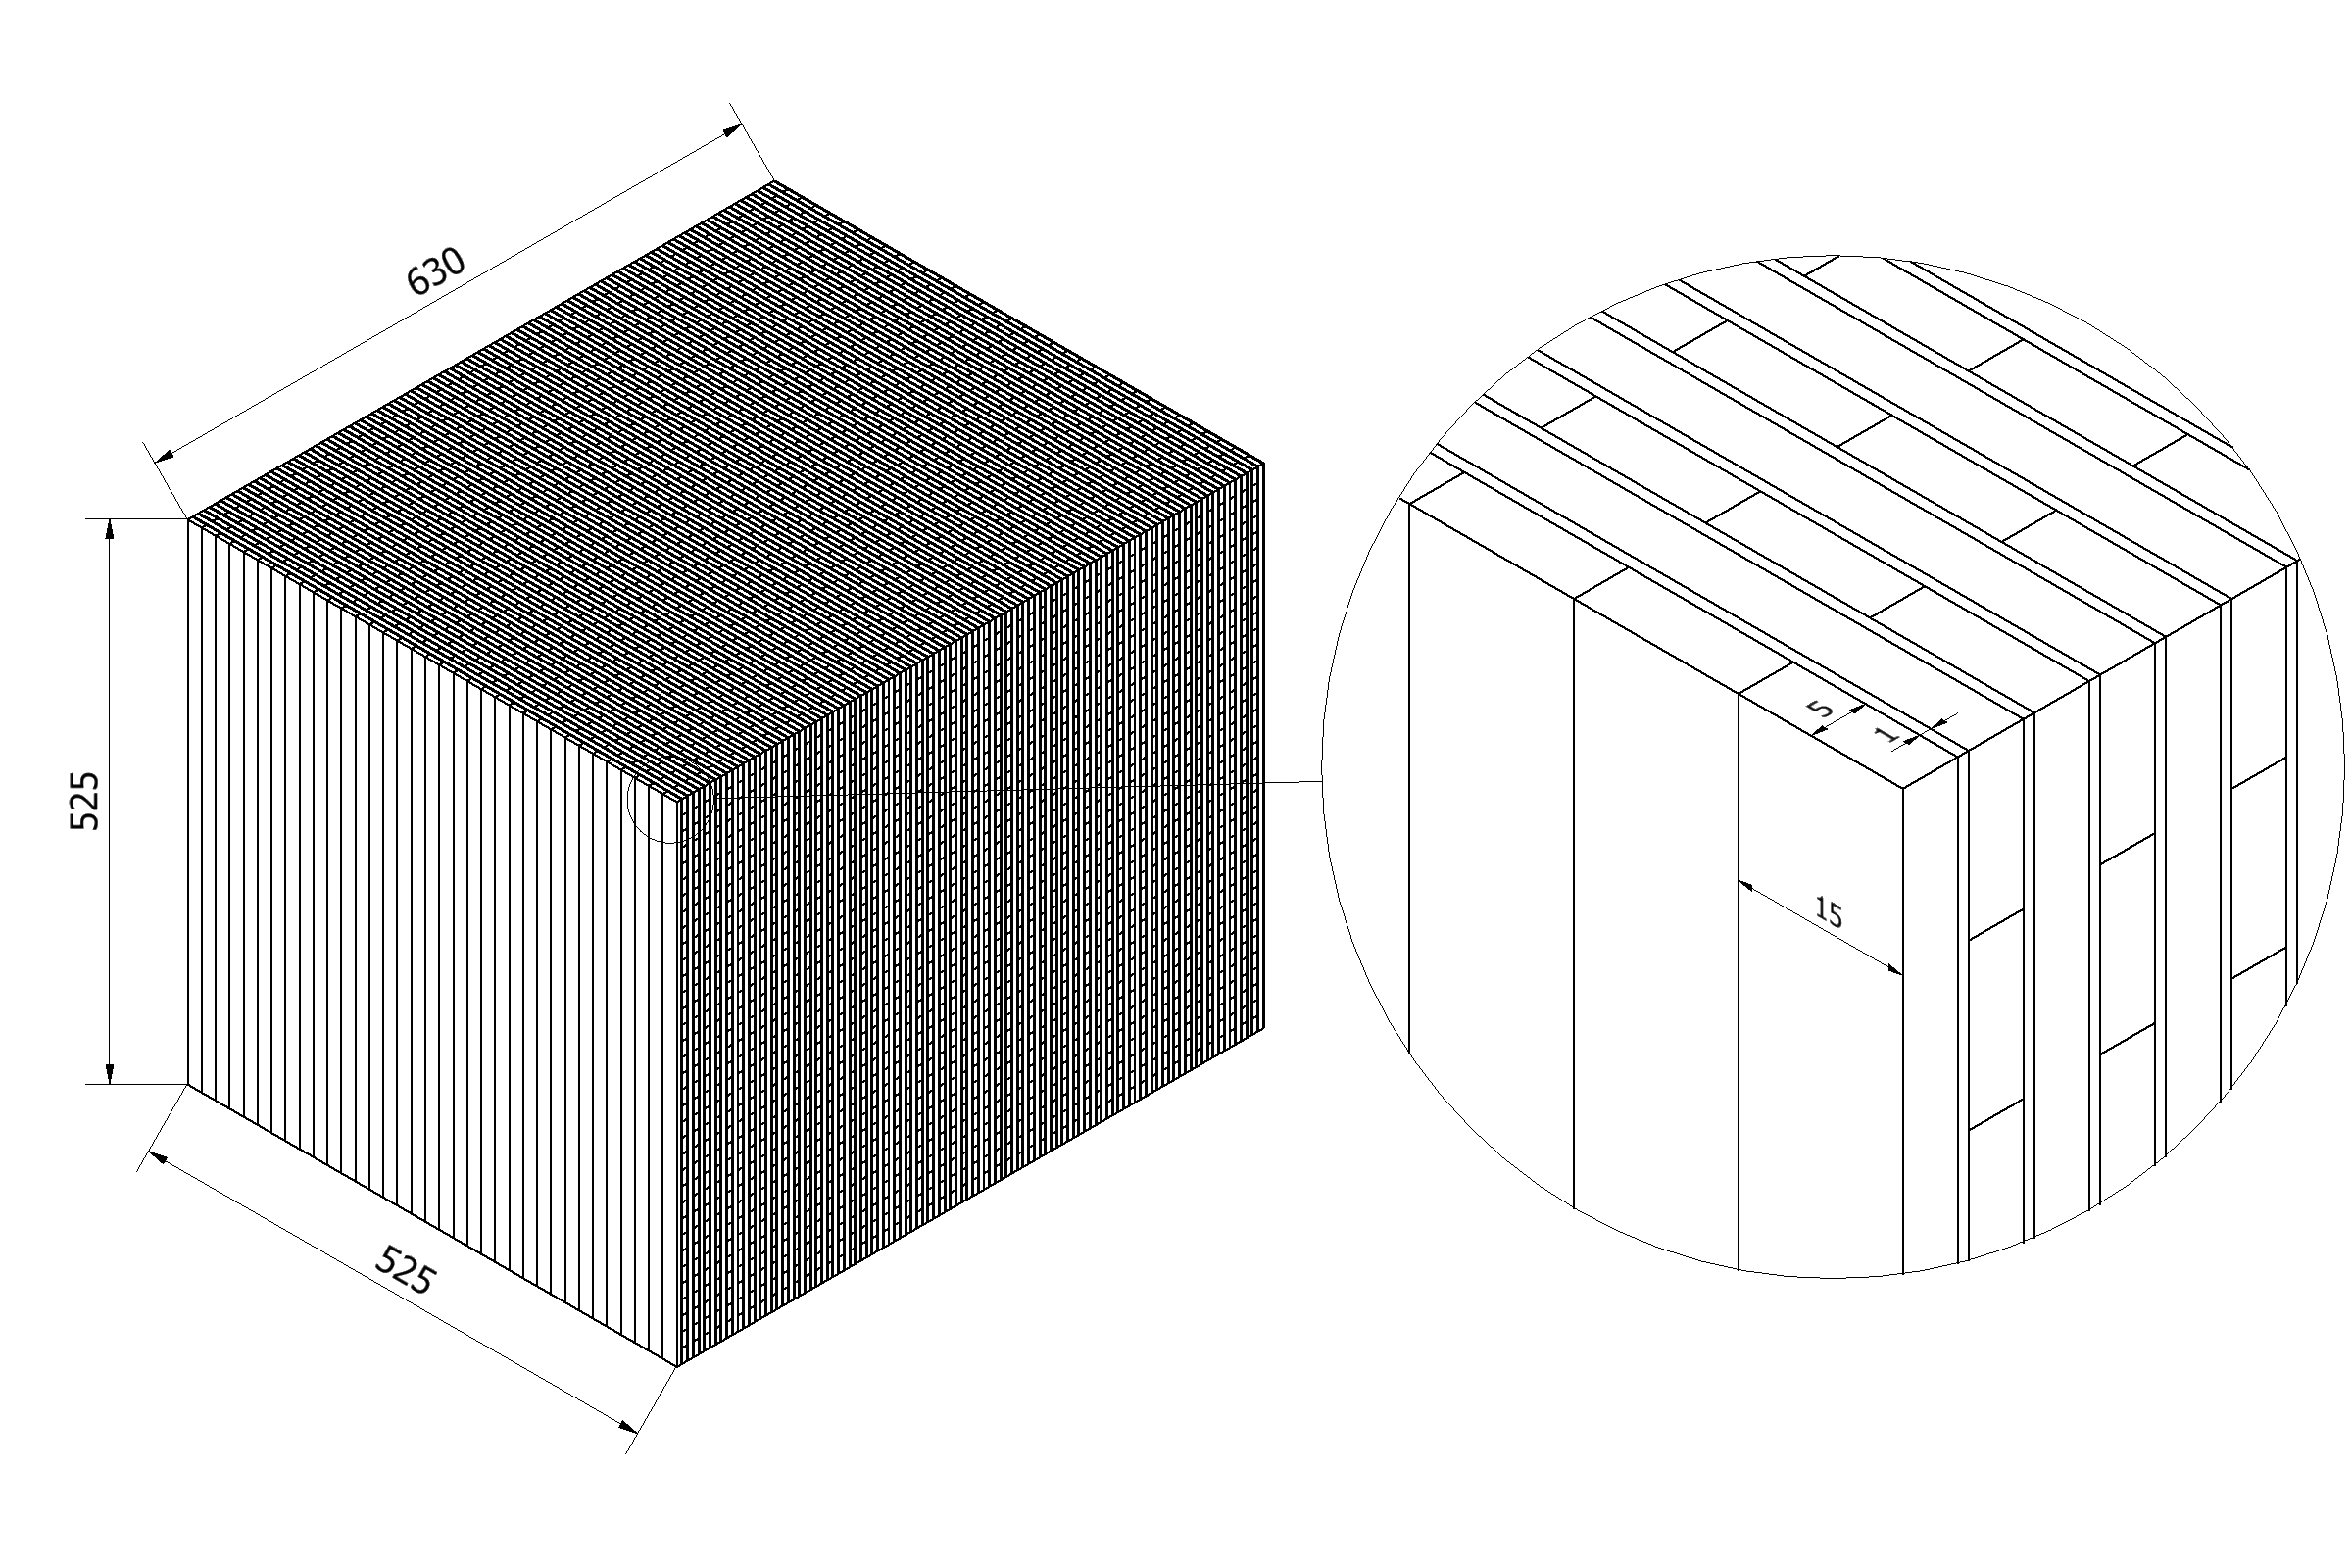
\includegraphics[width=0.6\textwidth]{figures/Fig1_detector_schematic.jpeg}
\caption{ Schematic of the sampling calorimeter model consisting of 105 alternating layers of a Pb and segmented scintillator plate in 35 strips. Each scintillator plate is oriented alternatively in horizontal and vertical directions. See text for details. }
\label{fig:det_conf}
\end{figure}


The sampling calorimeter was designed as a block consisting of alternating layers of an 1-mm-thick Pb absorber and a 5-mm-thick polyvinyltoluene-based plastic scintillator. The plastic scintillator is segmented into 15-mm-wide strips, which are alternatively oriented in the vertical and horizontal directions, as shown in Figure~\ref{fig:det_conf}. It has a cross-section of size 525~$\times$~525~mm$^{2}$ and accommodates 105 alternating layers of 630~mm length, which corresponds to 20 radiation lengths (20$X_{0}$) that are sufficiently long to absorb full photon energy in the range of 0.1 to 2~GeV.

\begin{figure}[!hbt]
\centering
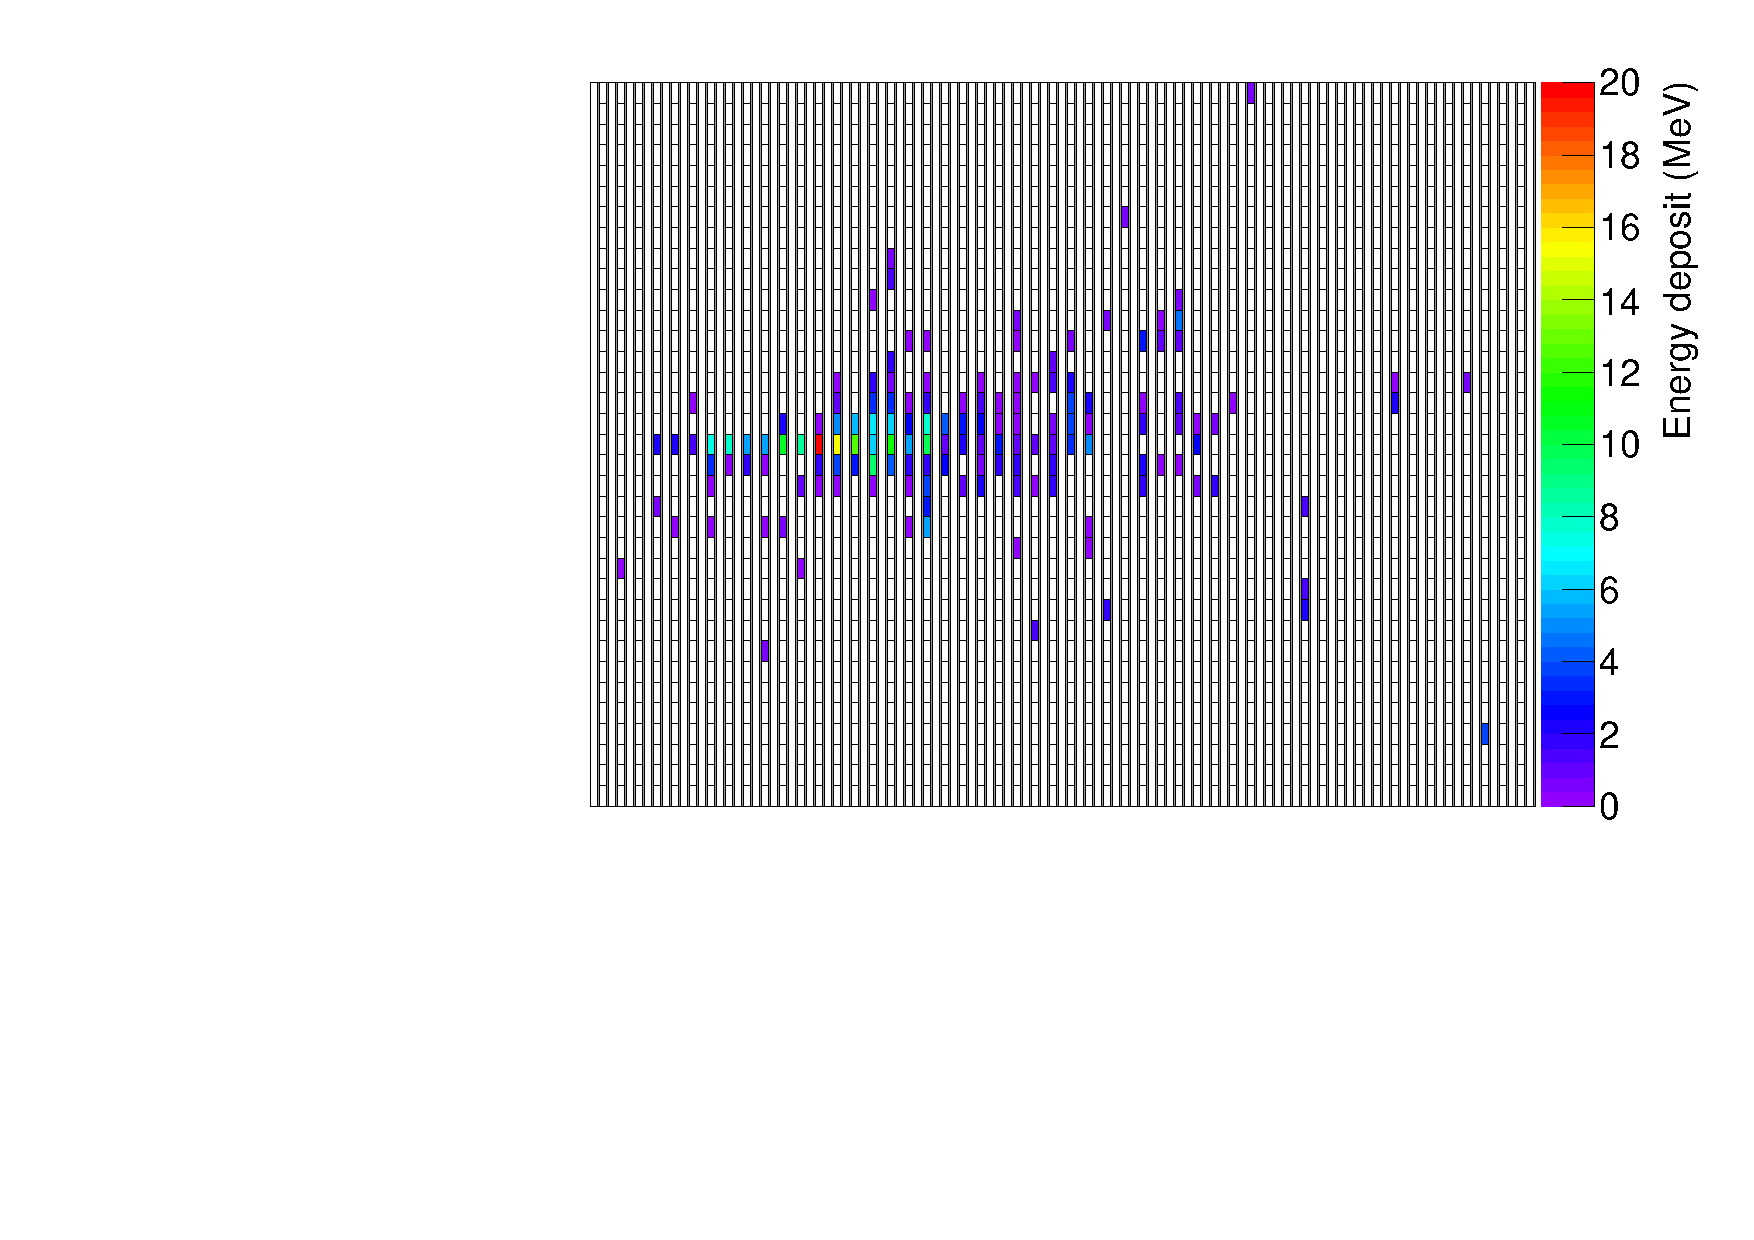
\includegraphics[width=0.48\textwidth]{figures/Fig2_EMShower_XZ.pdf}
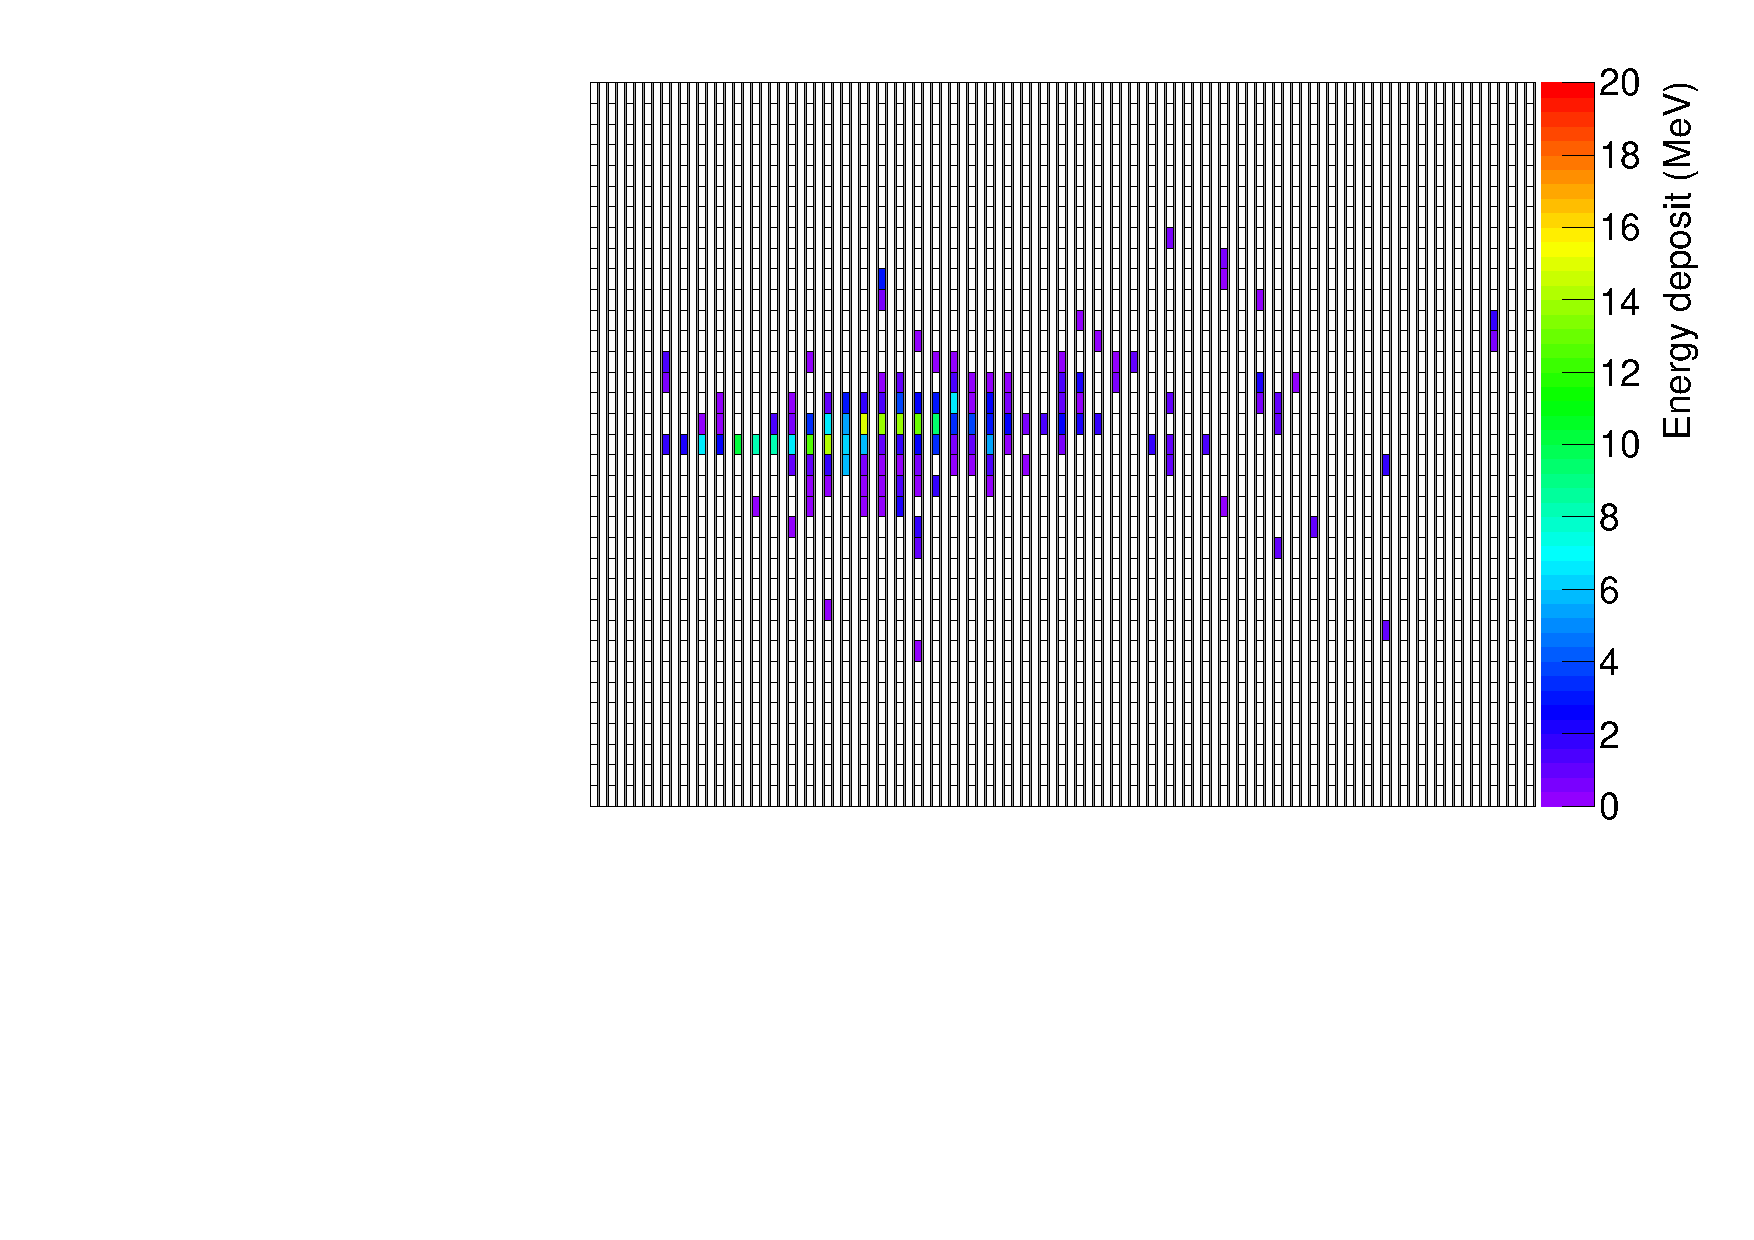
\includegraphics[width=0.48\textwidth]{figures/Fig2_EMShower_YZ.pdf}
\caption{ Event display of simulated energy deposit patterns for an 1-GeV photon entering the calorimeter ($\theta=$~0) in (a) $xz$- and (b) $yz$-planes.}
\label{fig:Evt_Dis}
\end{figure}



The detector response to the incident photons was simulated using Geant4 (ver. 4.10.06) with standard EM sub-packages~\cite{GEANT4}. The direction normal to the detector surface defines the $z$-axis. The photon direction was defined by the polar angle ($\theta$) with respect to the $z$-axis. Figure~\ref{fig:Evt_Dis} illustrates the simulated energy deposit patterns in each strip for an 1-GeV photon at normal incidence in the $xz$- and $yz$-planes. Each segmented region shown in Figure~\ref{fig:Evt_Dis} represents a channel.

\section{Reconstruction of Incident Angles}
\label{sec:res}

The incident angles of the photons are reconstructed using XGB~\cite{xgboost:2016}, which maps a feature dataset of the energy deposits in each scintillator strip onto a target variable, the incident angle of a photon. Training data were carefully prepared using the Geant4 simulation such that the input datasets were representative of the detector response of the real sampling calorimeters. To minimize the bias in the training process related to the dataset, the incident angles were uniformly generated at the detector surface in the angular range of 0~$<\theta<$~50$^{\circ}$ and 0~$<\varphi<$~360$^{\circ}$, where $\varphi$ denotes the azimuthal angle. The number of training samples was $10^{5}$ considering the limited computing resources. To test the reconstruction of the incident angles, we generated photons at a fixed incident angle $\theta$ with a known incident energy.

\begin{figure}[!hbt]
\centering
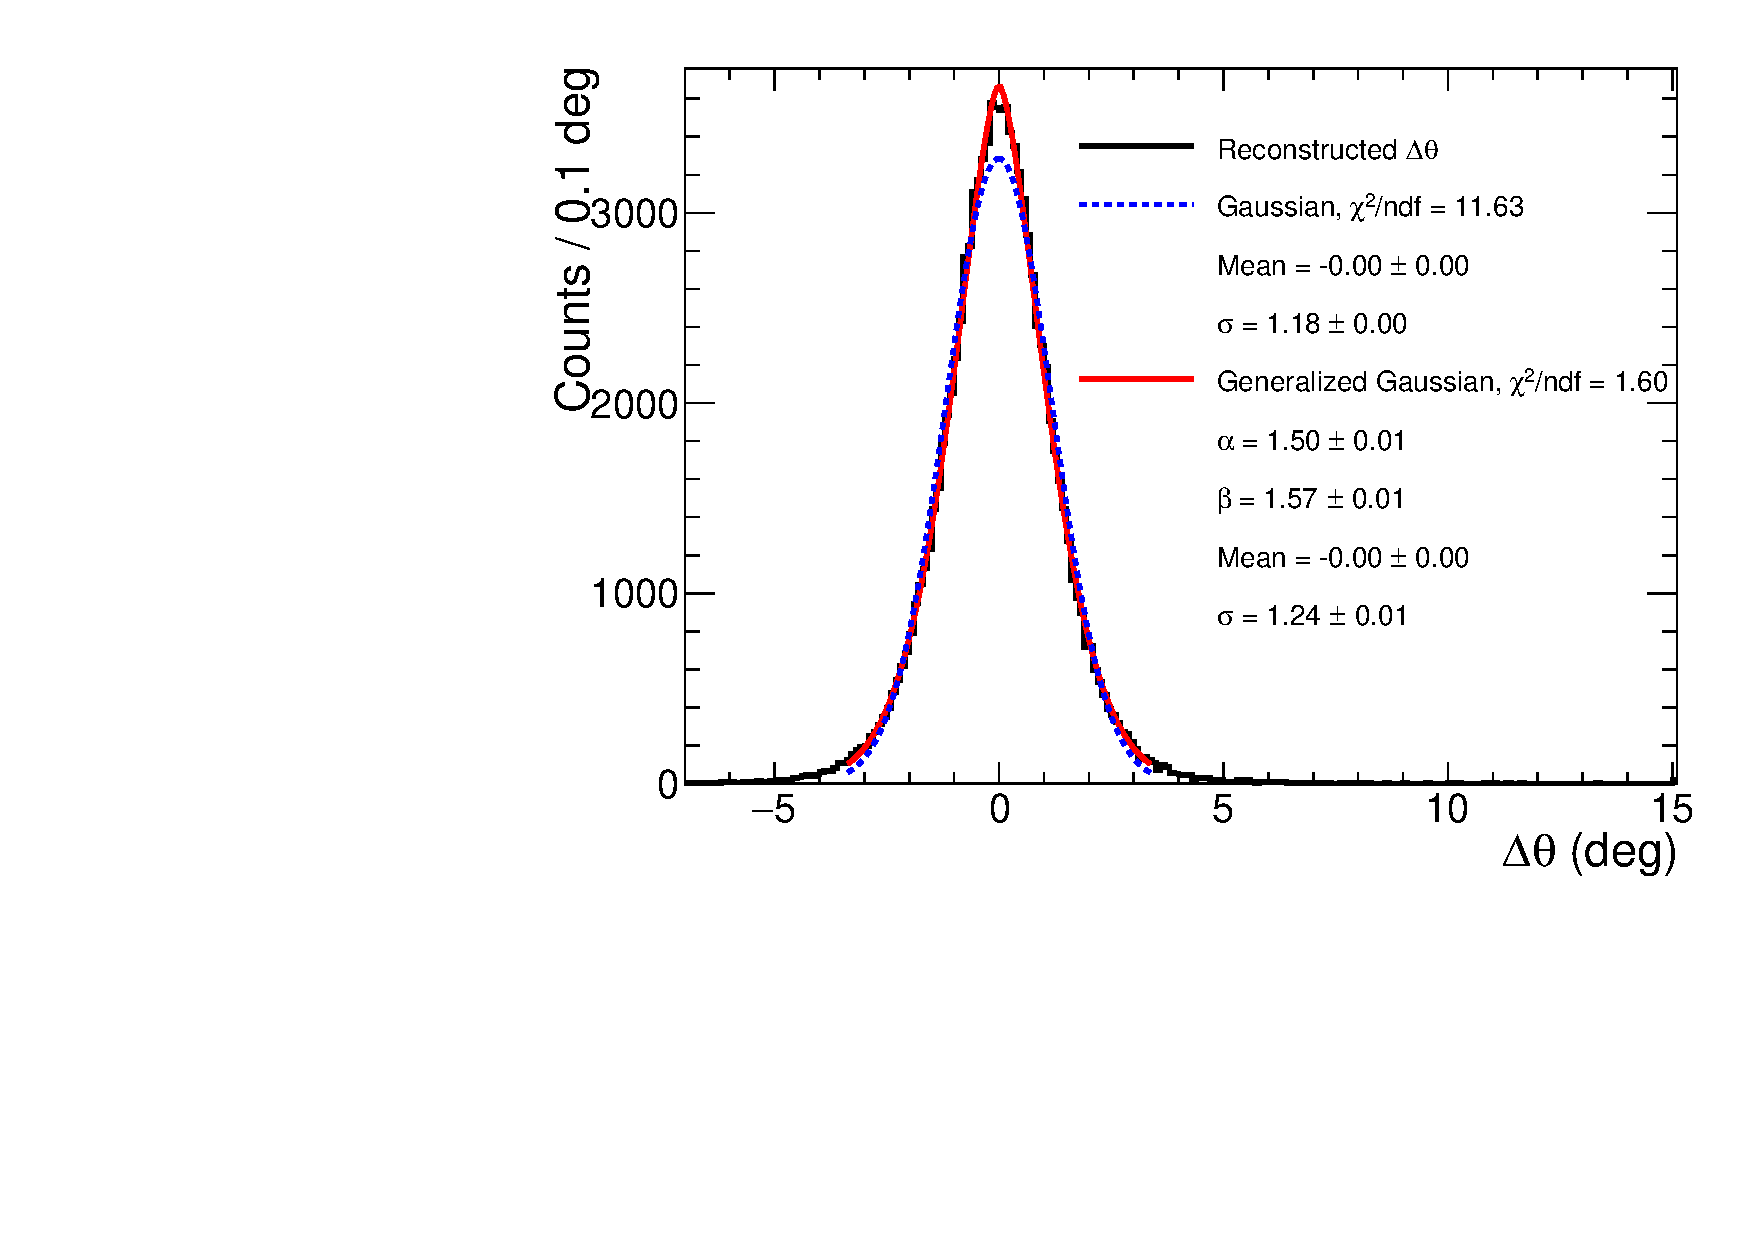
\includegraphics[width=0.7\textwidth]{figures/Fig3_fit_GG.pdf}
\caption{ The relative incident angle for 1-GeV photons generated at $\theta=$~10$^{\circ}$. The distribution is fitted with the Gaussian and generalized Gaussian functions. The generalized Gaussian function gives a better result.}
\label{fig:angle_10degree}
\end{figure}

Figure~\ref{fig:angle_10degree} represents the distribution of the relative incident angle ($\Delta\theta$) for 1-GeV photons generated at $\theta=$~10$^{\circ}$. $\Delta\theta$ represents the radial displacement of the reconstructed incident angle relative to the true incident direction. The central 98\% of the distribution is fitted with the Gaussian and generalized Gaussian (GG) functions~\cite{GGfun}. We tested two functions, Gaussian and GG, to describe the reconstructed angular distribution. The GG function, also known as the generalized error distribution, is expressed as:
\begin{eqnarray} 
f(x; \mu, \alpha, \beta) = \frac{\beta}{2 \alpha \Gamma(1/\beta)}e^{-(|x-\mu|/\alpha)^\beta},
\label{eqn:gg}
\end{eqnarray}
where $\mu$ is the mean value. The parameters $\alpha$ and $\beta$ determine the scale and shape of the distribution, respectively. The variance in the GG function is given by $\sigma^2 \equiv \alpha^2 \Gamma(3/\beta) / \Gamma(1/\beta)$. The angular resolution of the incident angle reconstruction is defined as $\sigma$.

\begin{figure}[!hbt]
\centering
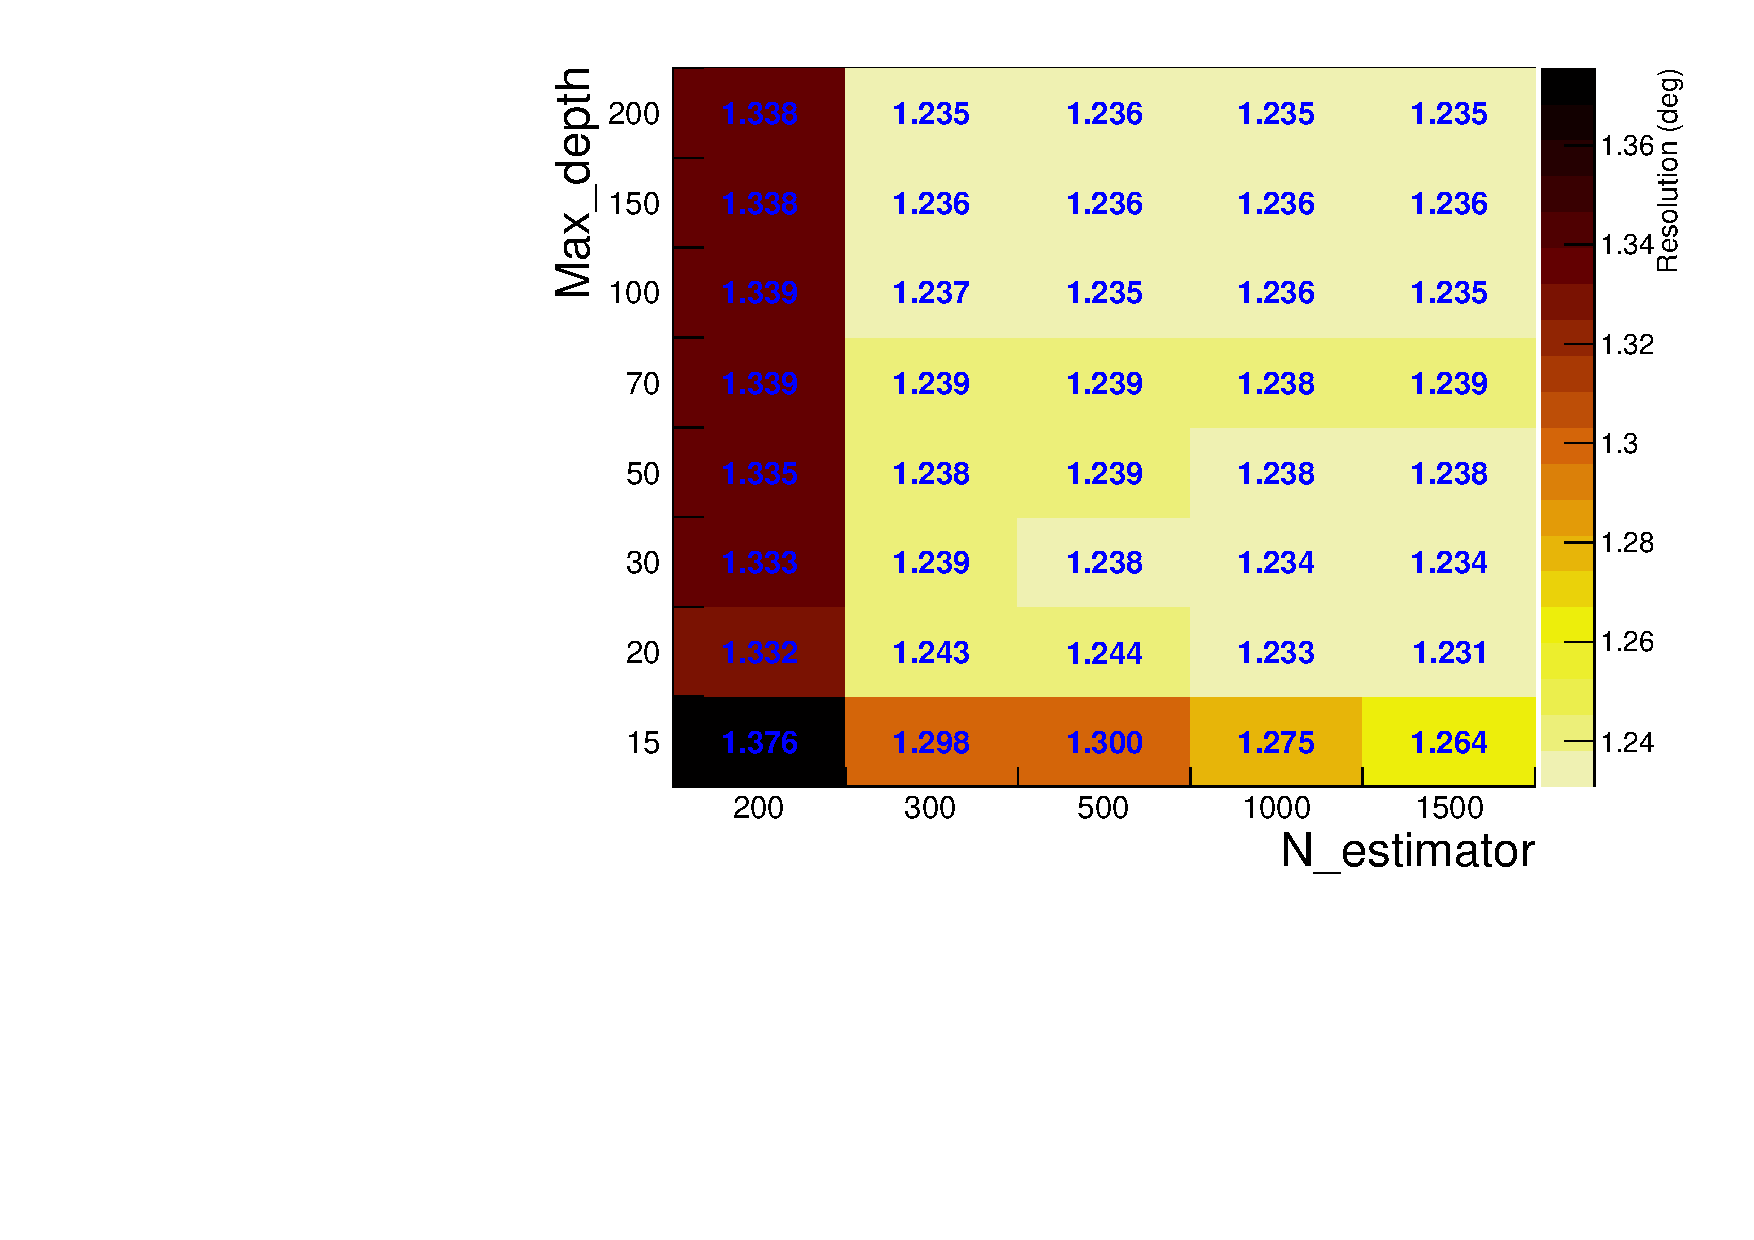
\includegraphics[width=0.69\textwidth]{figures/Fig4_Opt.pdf}
\caption{Angular resolutions are displayed in terms of combination of N\_estimators and Max. depth. The best angular resolution is obtained with N\_estimators~=~300 and Max. depth~=~100. }
\label{fig:par_scan}
\end{figure}

Because the performance of the angle reconstruction of the XGB depends on the hyperparameters, we scanned the evaluated angular resolution by changing the hyperparameters. As there were correlations among the hyperparameters, the scanning process was performed in a five-dimensional space for all possible combinations. As an example, Figure 4 shows the test results for N\_estimators and Max. depth. N\_estimators defines the maximum allowed number of decision trees to be developed, and Max. depth defines the complexity of the decision-tree structure. We explored a hyperparameter combination that generated the best angular resolution. Consequently, the N\_estimators and Max. depth were set to 300 and 100, respectively. Similar scans were also performed for different hyperparameters, subsample, learning rates, and gamma. Subsample controls the fraction of total event samples for each boosting procedure, the learning rate weights a decision tree to be added onto the current model, and the gamma regulates the evaluation of each decision tree. Table~\ref{tab:XgbPar} lists the optimized set of hyperparameters that are used in further studies. During the optimization process, the fraction of the tail that is not well described by the GG function is approximately 2\%.

\begin{table}[hbt!]{\small
\centering
\caption{Hyperparameters of the XGB model}
\begin{tabular}{cccc}
\hline 
Parameter & Function & Default value & Used value \\ \hline 
N\_estimators & The number of decision trees & N.A. & 300 \\  
Max. depth & Possible maximum depth of tree structure & 6 & 100 \\ 
Subsample & Fraction of total data used for a single decision & 1 & 0.8 \\ 
Learning rate & Step length for calculation & 0.3 & 0.02 \\ 
Gamma & Requirement on minimum loss function & 0 & 0 \\ 
\hline
\end{tabular}
\label{tab:XgbPar}
}\end{table}

\begin{figure}[!hbt]
\centering
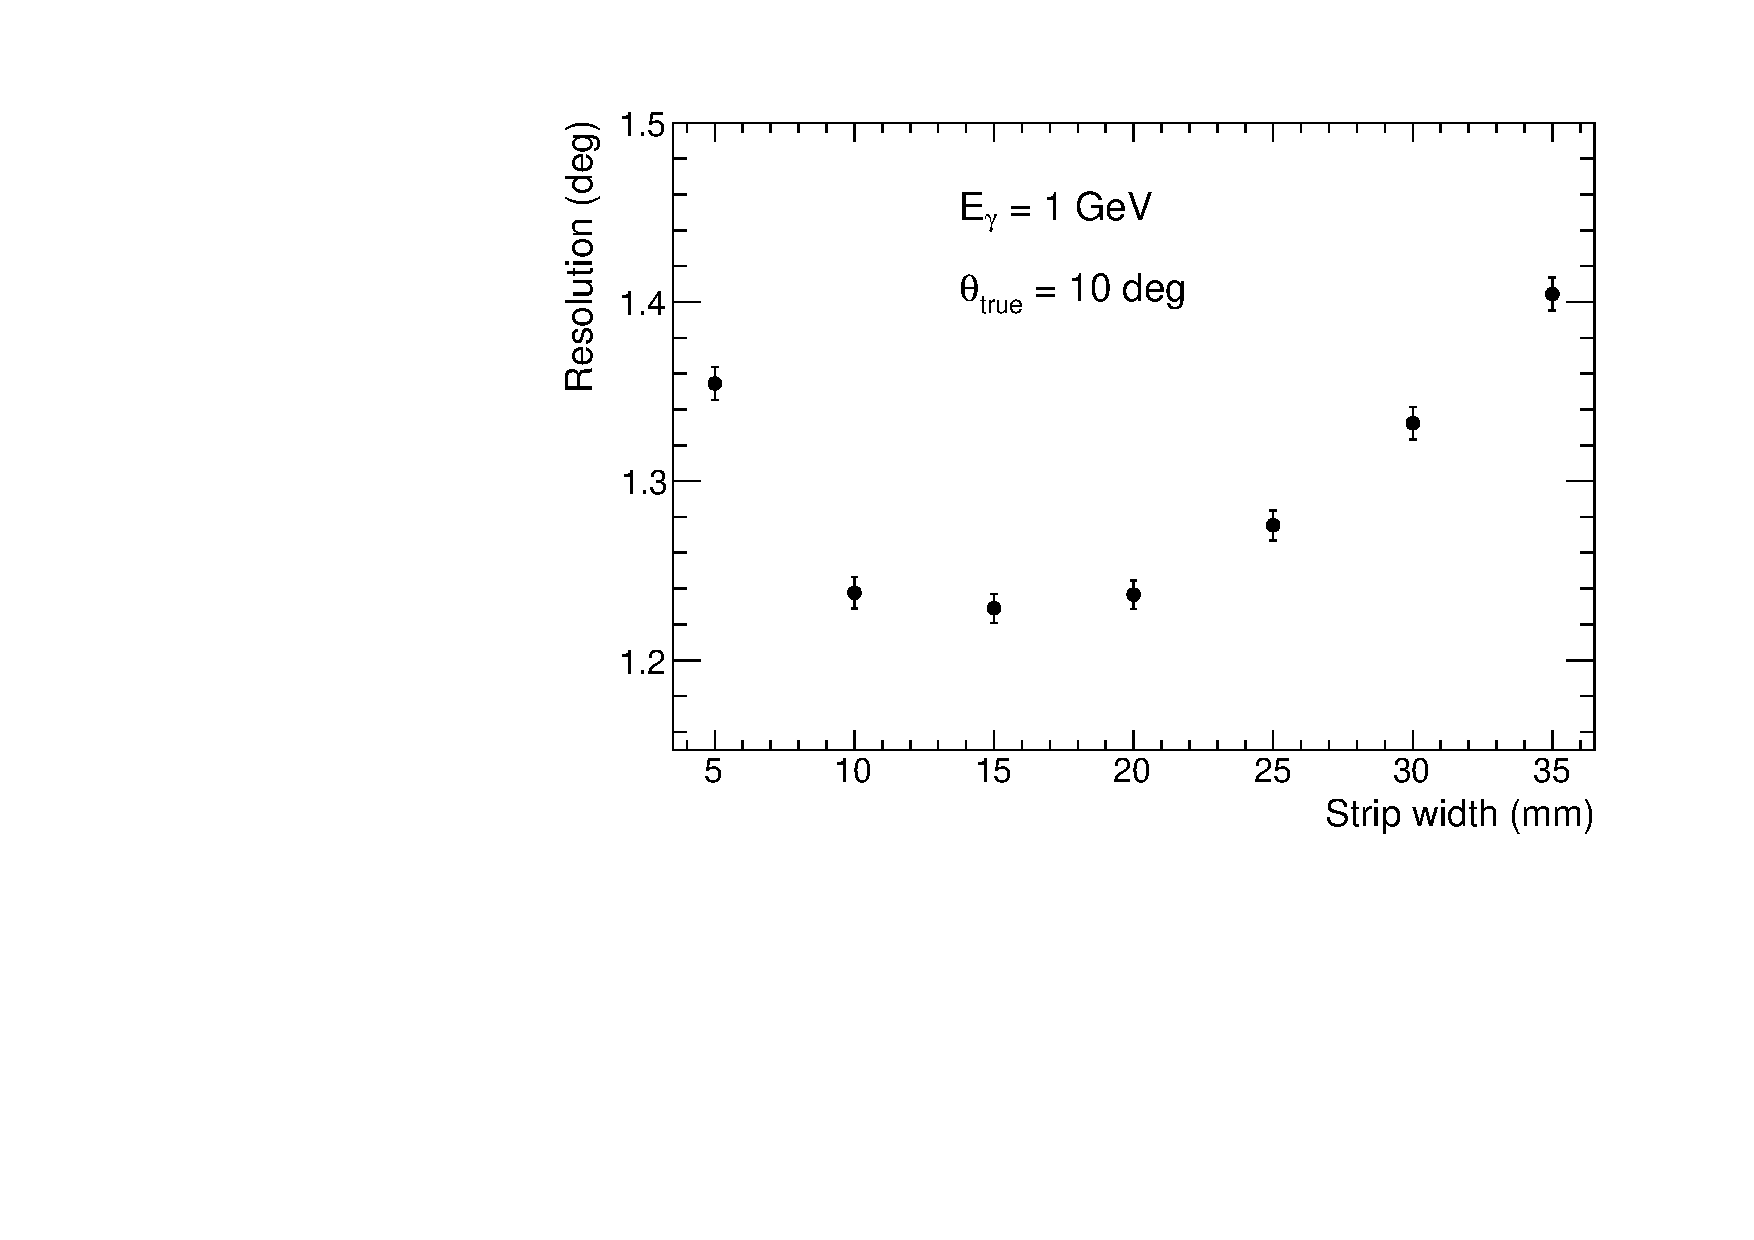
\includegraphics[width=0.58\textwidth]{figures/Fig5_width.pdf}
\caption{ Angular resolutions are deduced in terms of the strip width for 1-GeV photons at $\theta=$~10$^{\circ}$ }
\label{fig:angle_reco_width}
\end{figure}

Angular resolutions were deduced by varying the strip width from 5 to 35 mm, as shown in Figure~\ref{fig:angle_reco_width}. The narrower the strip width, the larger is the size of the features. Consequently, the angle-reconstruction performance declines. However, the wider strips hardly provide detailed information on the EM shower. The 15-mm-wide strips yield a good angular resolution of 1.23~$\pm$~0.01$^{\circ}$.

\begin{figure}[!hbt]
\centering
\stackinset{c}{0.cm}{b}{-0.4cm}{(a)}{
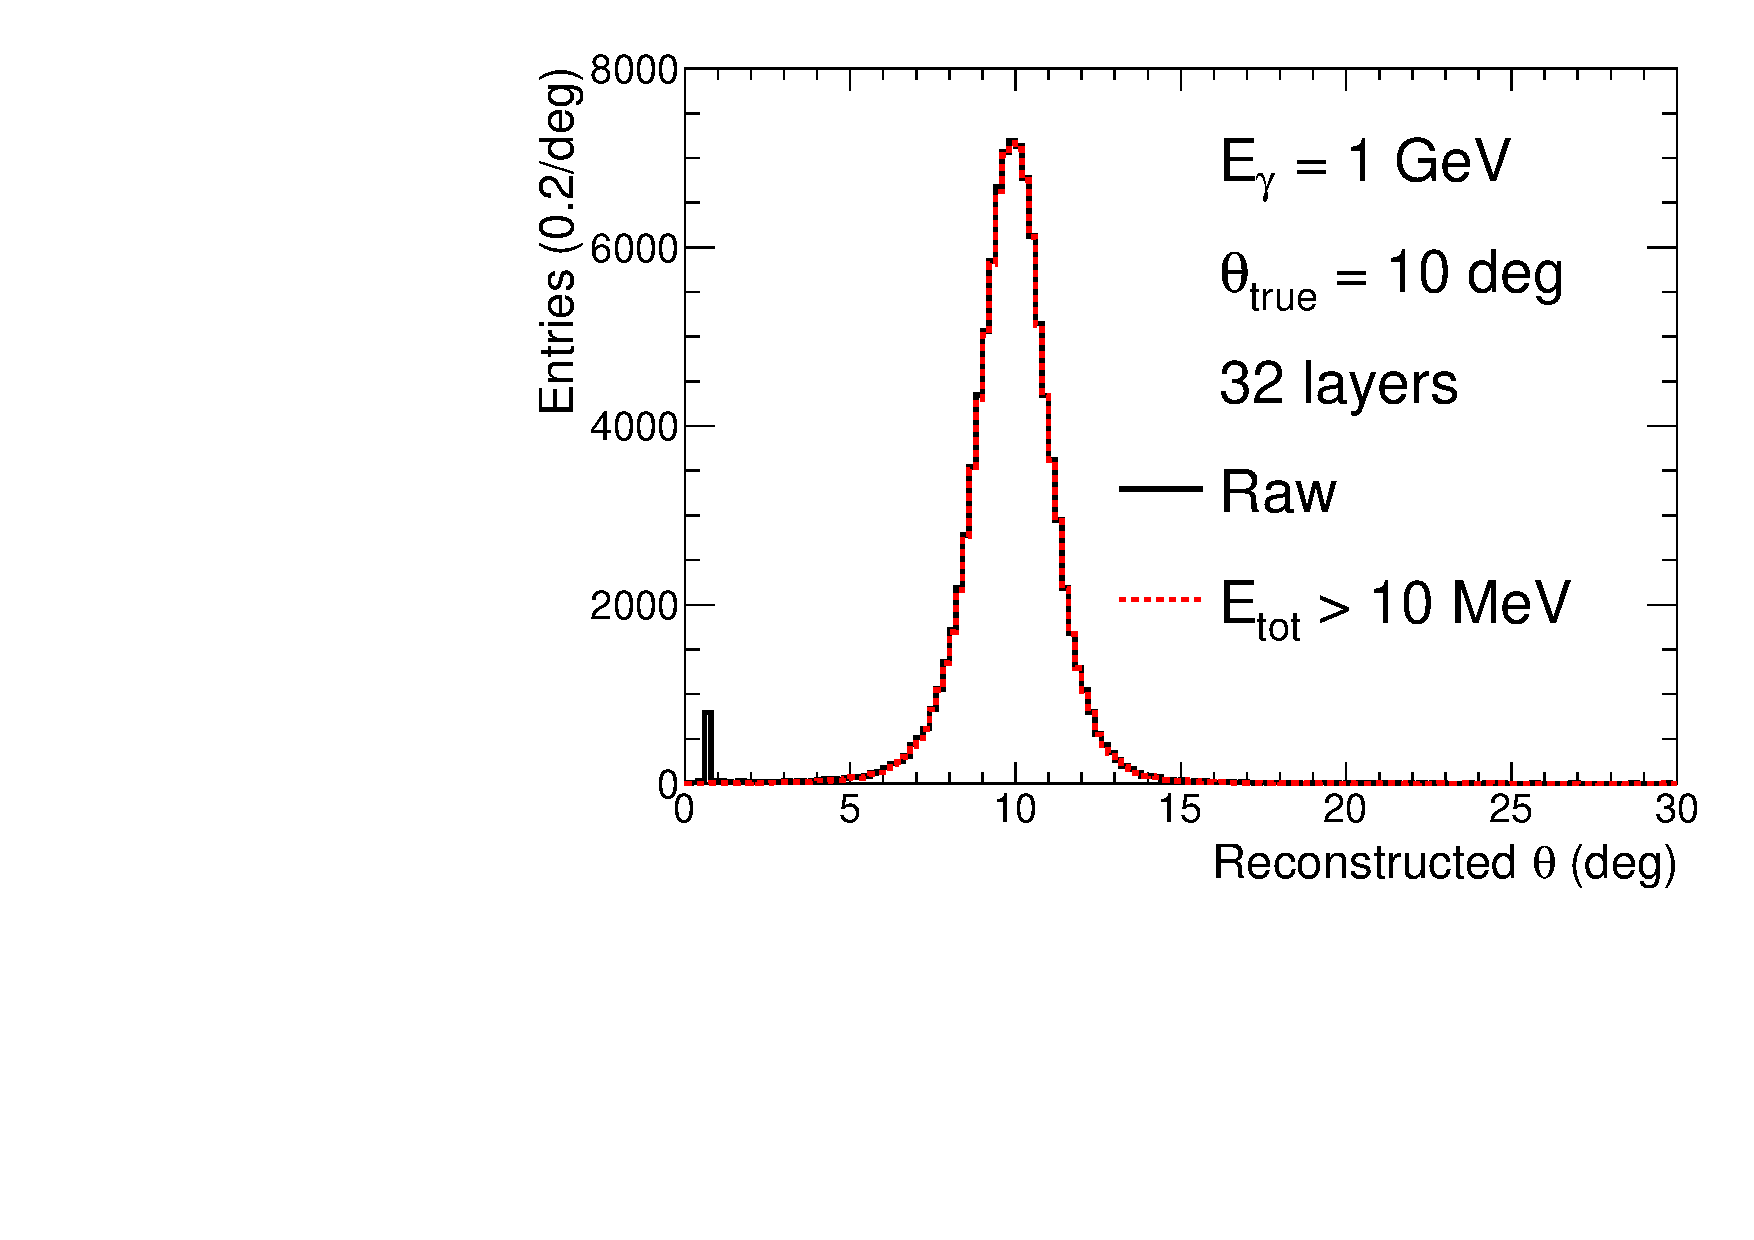
\includegraphics[width=0.48\textwidth]{figures/Fig6_layer_comp.pdf}
}\stackinset{c}{0.cm}{b}{-0.4cm}{(b)}{ 
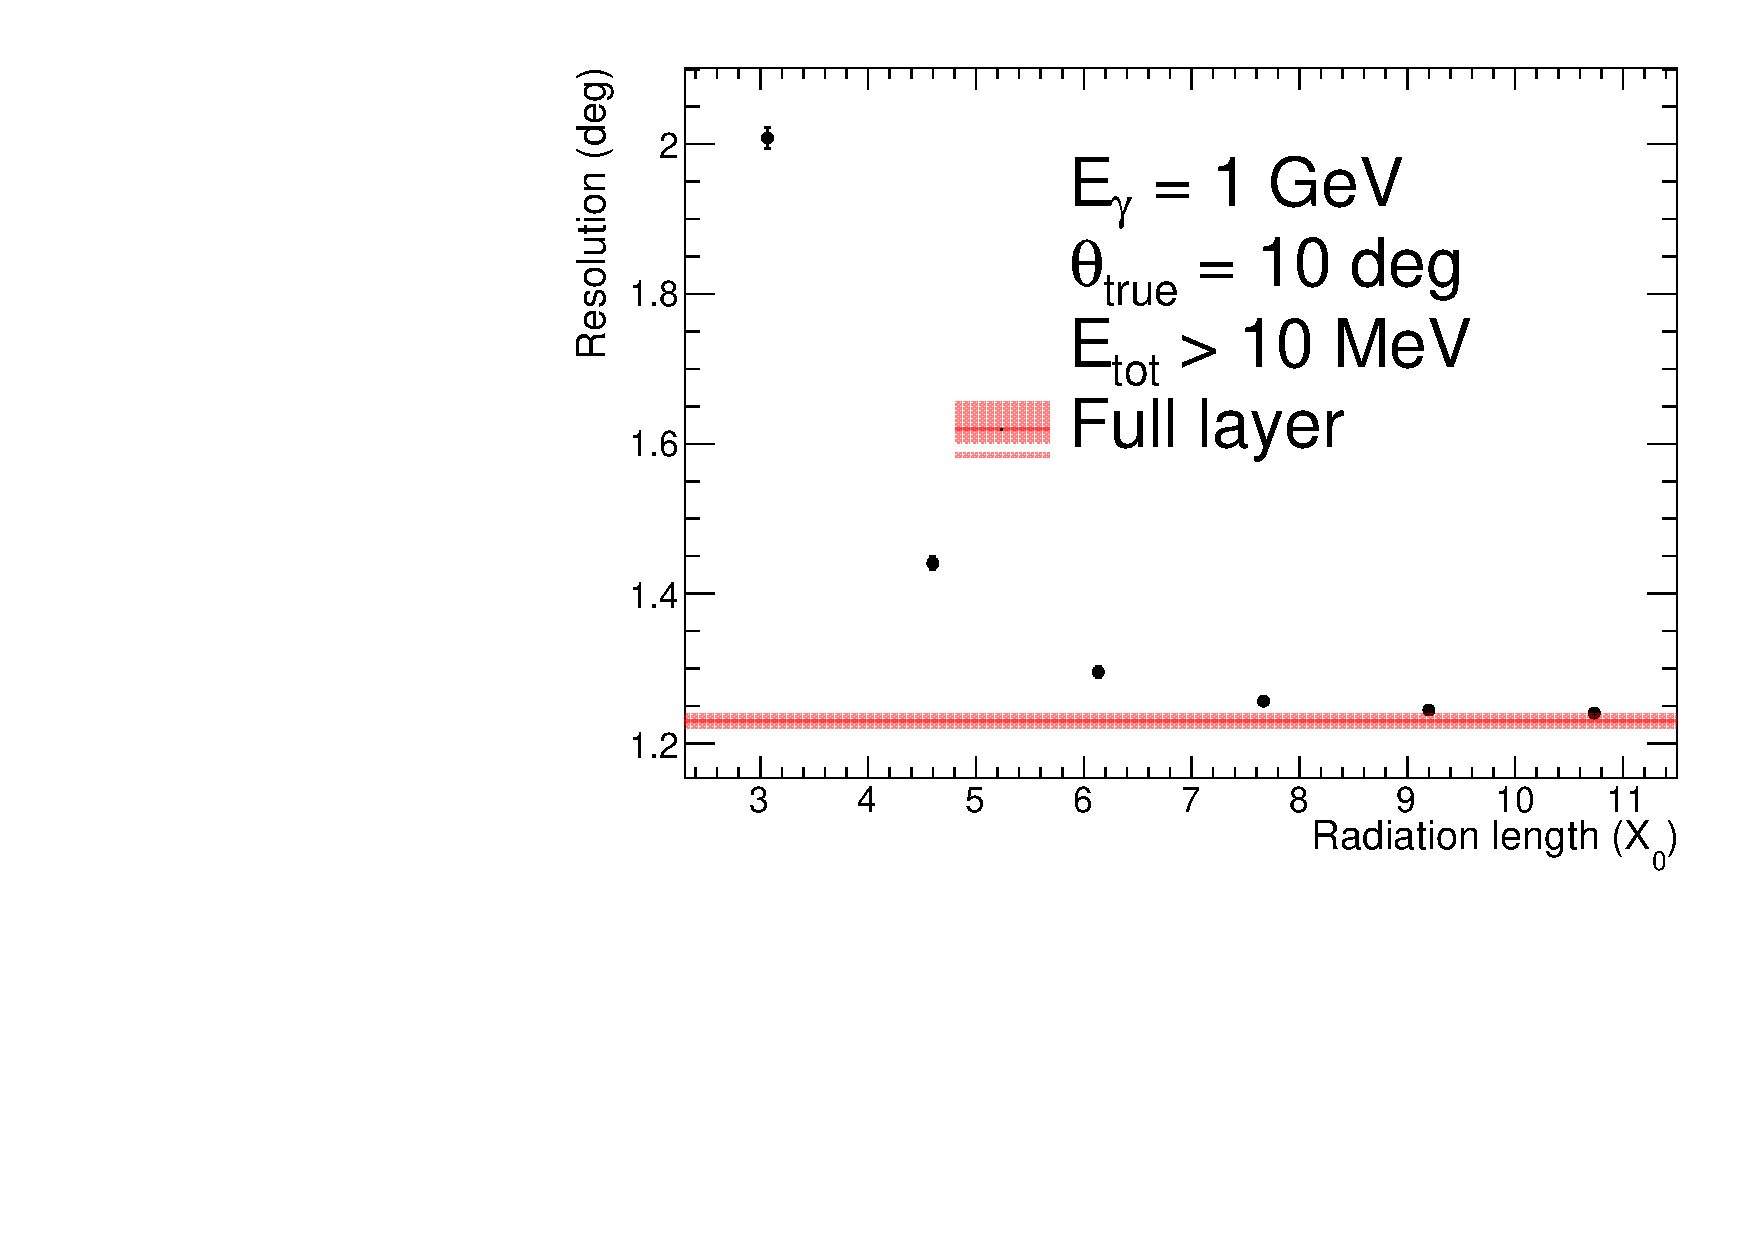
\includegraphics[width=0.48\textwidth]{figures/Fig6_nlayer.pdf}
}
\caption{ (a) Reconstructed polar angles ($\theta$) for 1-GeV photons at $\theta=$~10$^{\circ}$. The red histogram represents the polar angle distribution for $E_{\rm{tot}}>$~10~MeV. (b) Angular resolution as a function of the radiation length ($X_{0}$).}
\label{fig:angle_reco_layer}
\end{figure}

Focusing only on the angle reconstruction, we designed the detector with the smallest number of layers. Figure~\ref{fig:angle_reco_layer} (a) shows the angles reconstructed using the front 32 layers of the detector, which correspond to 6.2$X_{0}$, for 1-GeV photons. A fraction of the photons fail to be reconstructed because of insufficient information gathering caused by deeply penetrating photons without shower generation. The failed events are represented as a delta function near 0, and such events are removed by fixing the total energy deposit at a value higher than 10~MeV, which is 1\% of the incident energy. The angular resolution of the front layer is estimated to be 1.30~$\pm$~0.01$^{\circ}$ when 1.9\% of the photons fail to be reconstructed.

\begin{figure}[!hbt]
\centering
\stackinset{c}{0.cm}{b}{-0.4cm}{(a)}{
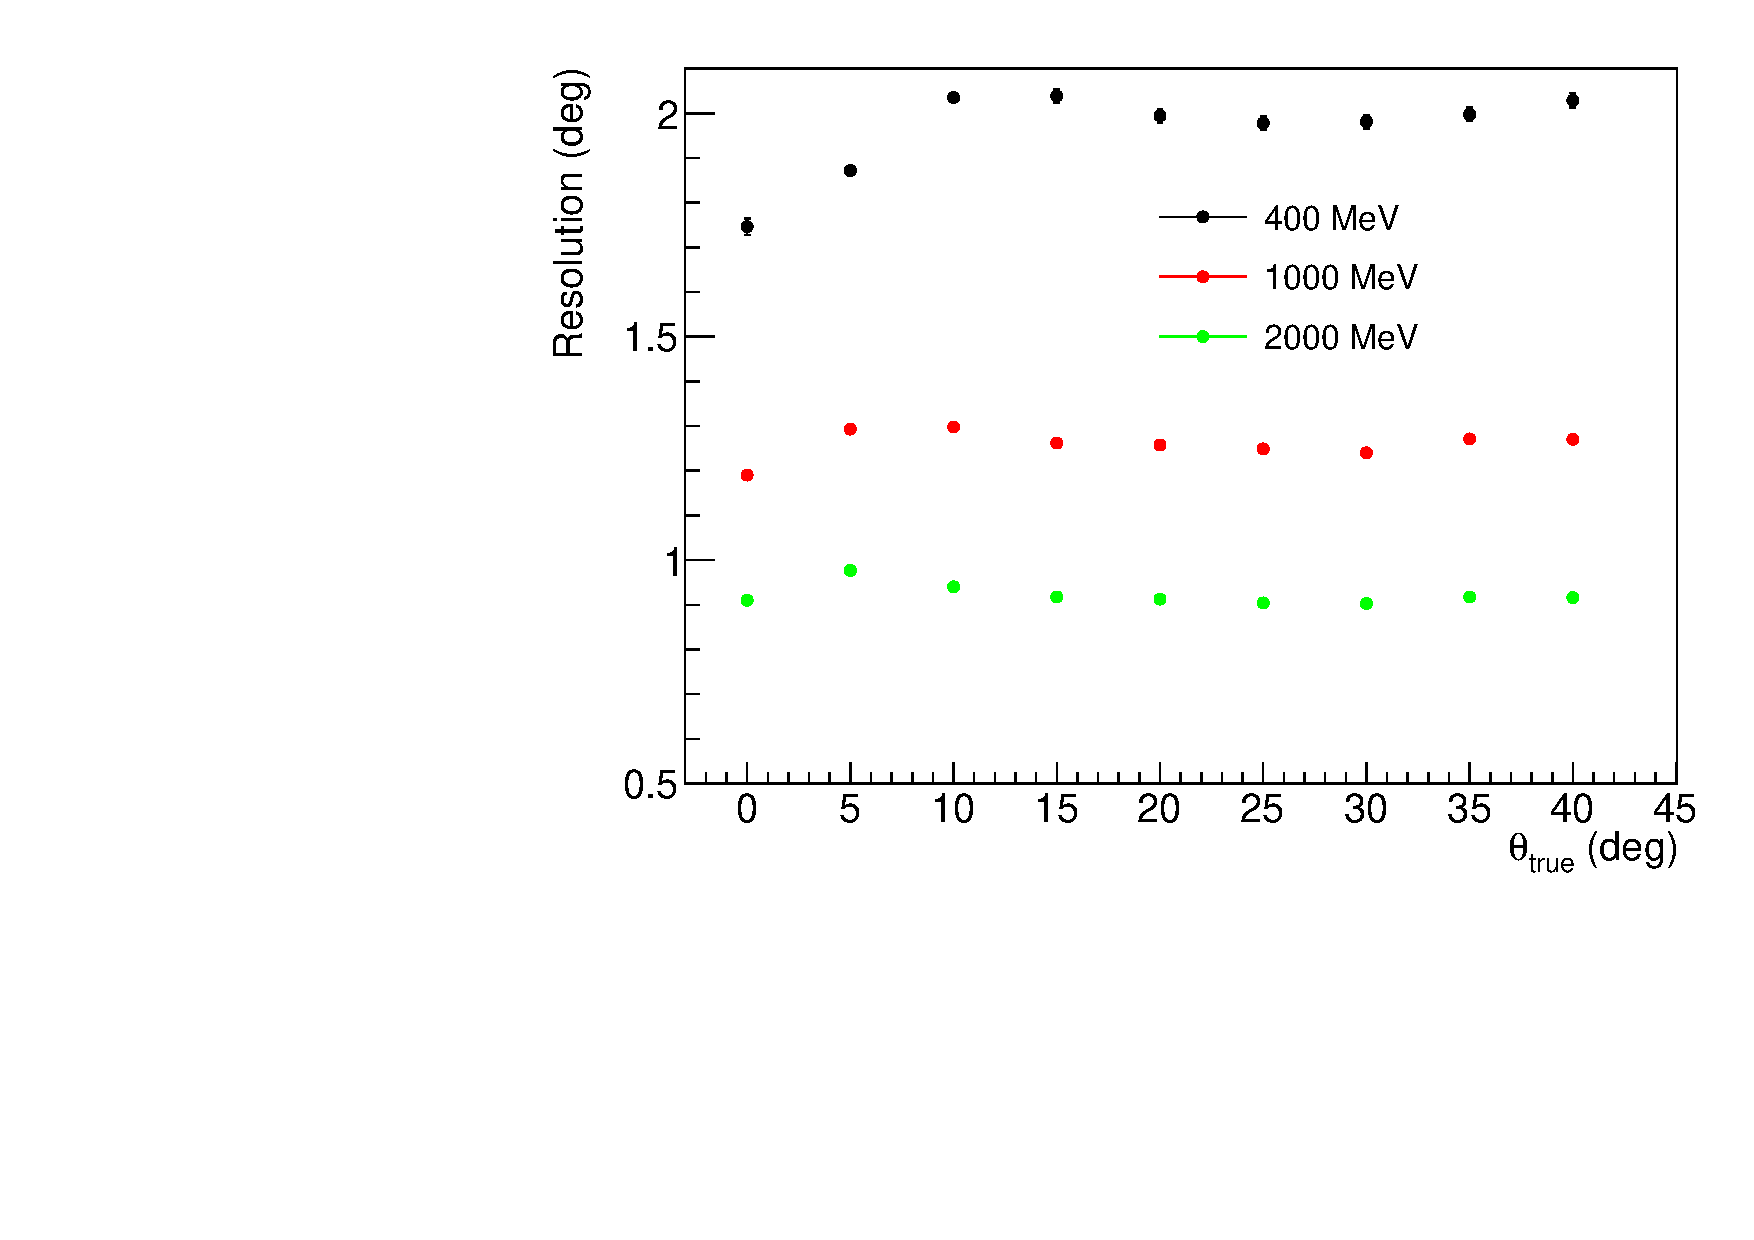
\includegraphics[width=0.44\textwidth]{figures/Fig7_res_ene.pdf}
}\stackinset{c}{0.cm}{b}{-0.4cm}{(b)}{
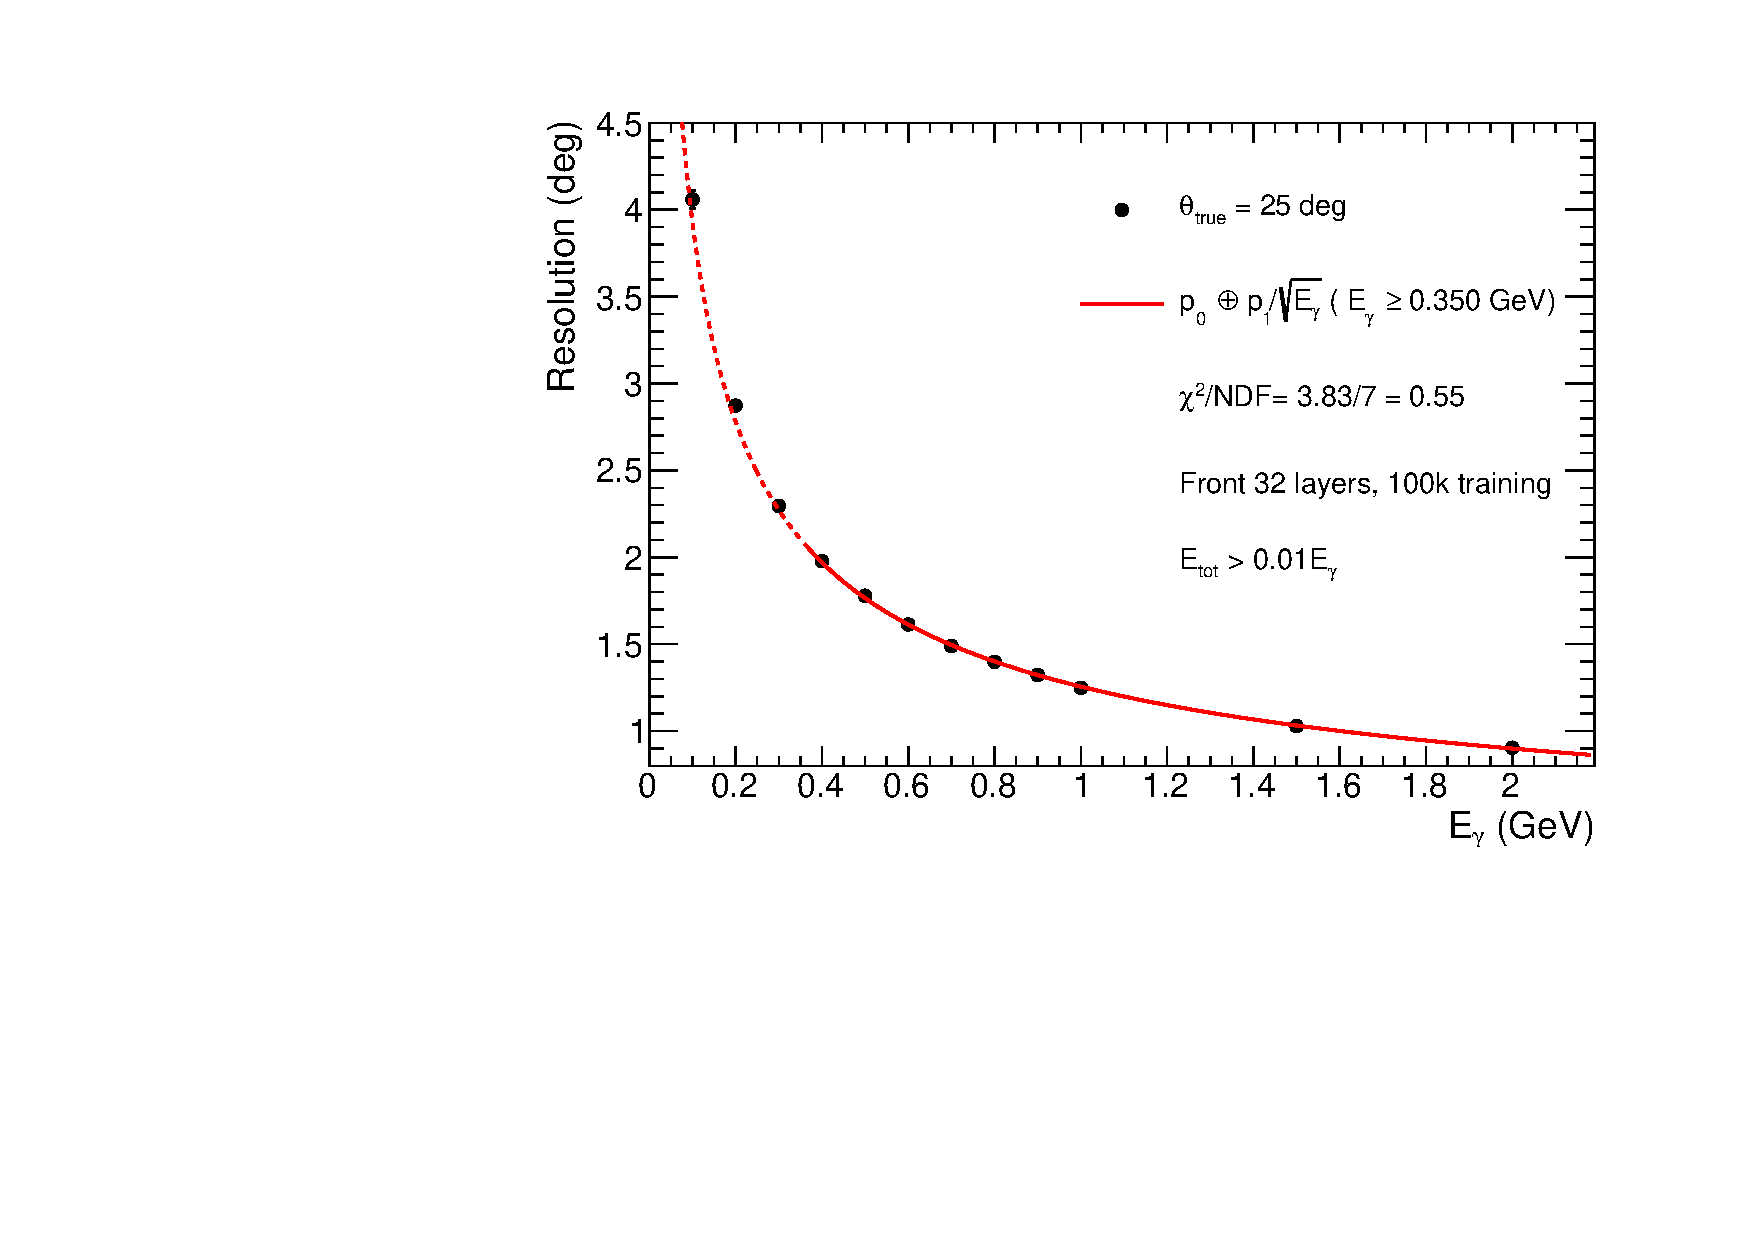
\includegraphics[width=0.44\textwidth]{figures/Fig7_Fit_eres_1.pdf}
}
\caption{ (a) Angular resolution as a function of the incident angle for different incident energies. (b) Angular resolution as a function of the incident energy for $\theta=$~25$^{\circ}$; it is fitted to the function $p_{0} \oplus p_{1}/\sqrt{E_{\gamma}(\mathrm{GeV})}$ }
\label{fig:angle_reco_dep_gr}
\end{figure}

Figure~\ref{fig:angle_reco_dep_gr} (a) shows the angular resolution as a function of incident angle for different incident energies ($E_{\gamma}$). The angular resolution does not depend on the incident angle for high incident energies. However, the angular resolution changes significantly for low incident energies at small incident angles. Figure~\ref{fig:angle_reco_dep_gr} (b) shows the angular resolution as a function of the incident photon energy at $\theta=$~25$^{\circ}$. The angular resolution fits to the function $p_{0} \oplus p_{1}/\sqrt{E_{\gamma}(\mathrm{GeV})}$, where $p_{0}$ and $p_{1}$ represent the energy-independent and energy-dependent contributions, respectively.

\begin{figure}[!hbt]
\centering
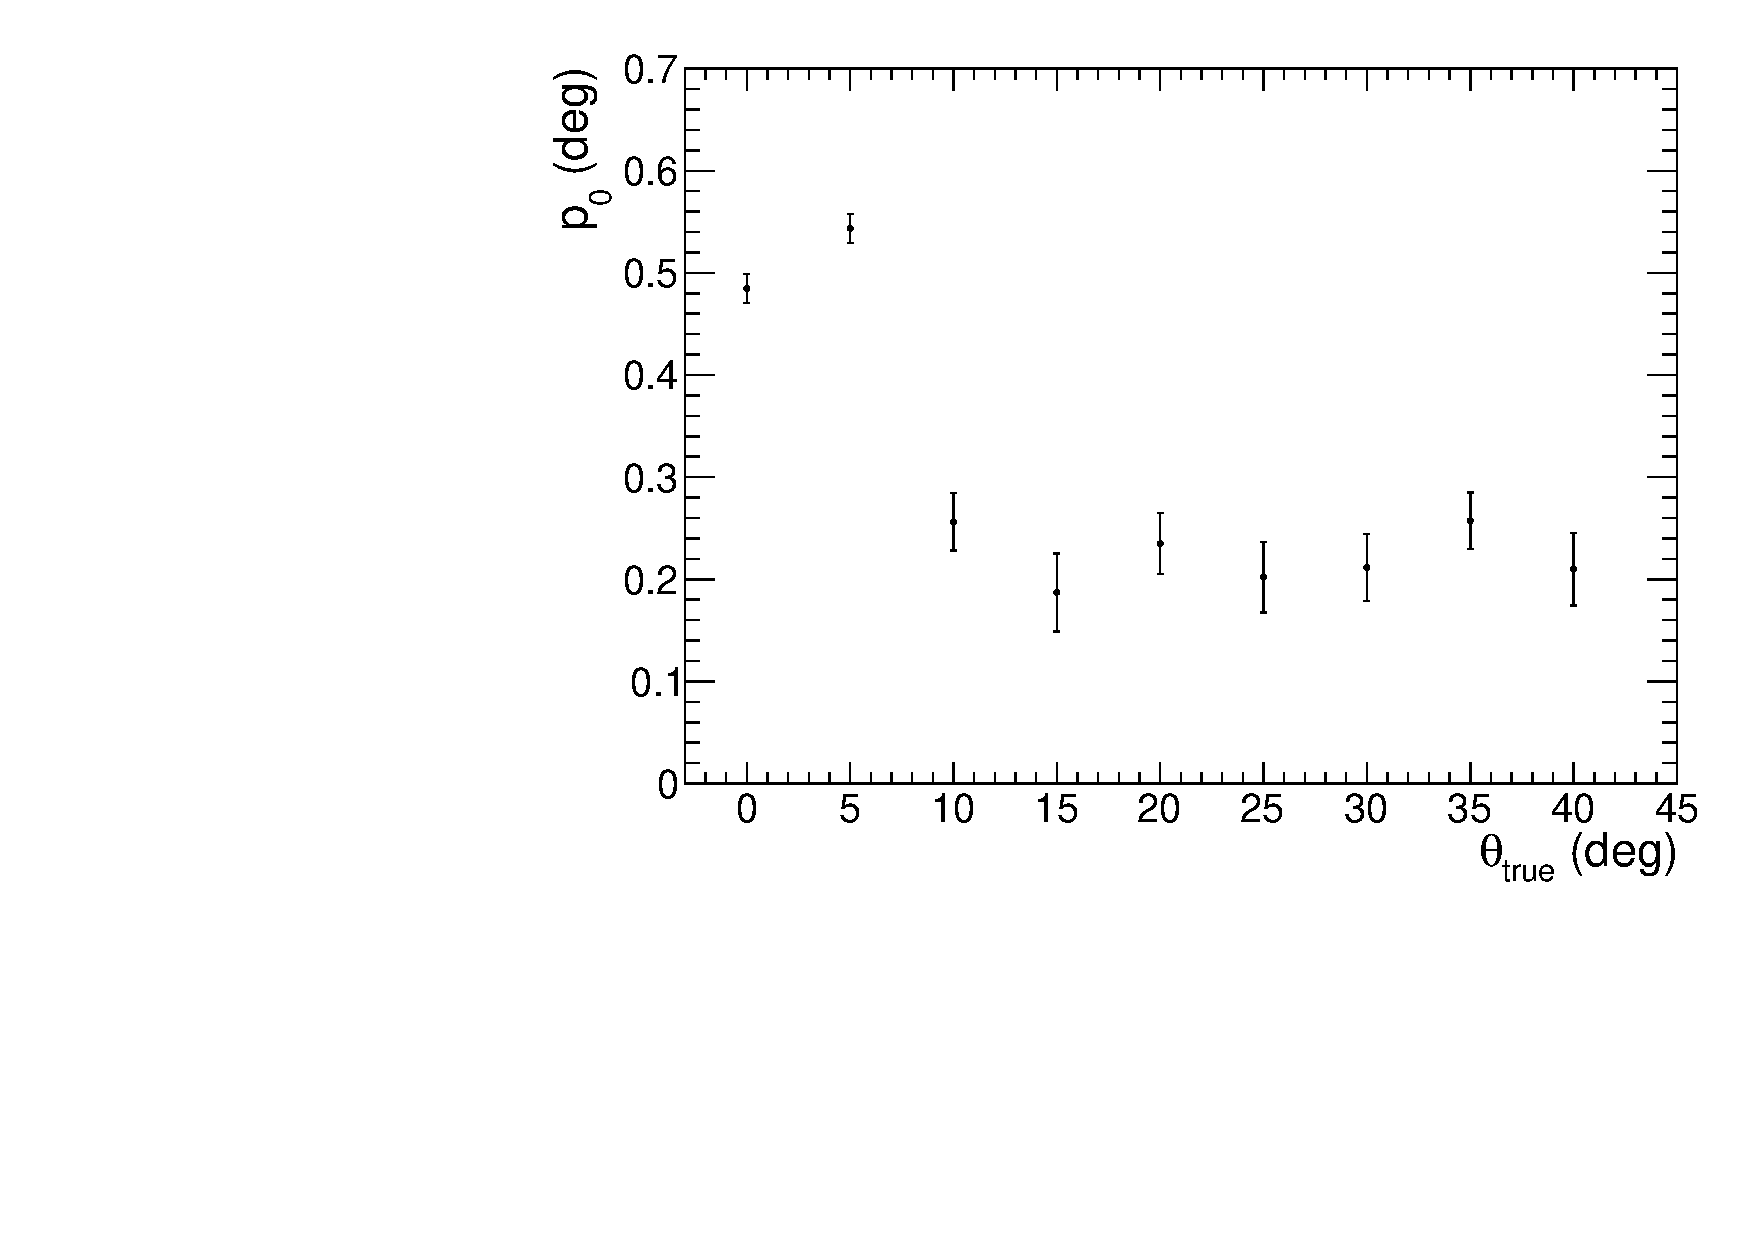
\includegraphics[width=0.44\textwidth]{figures/Fig7_p0.pdf}
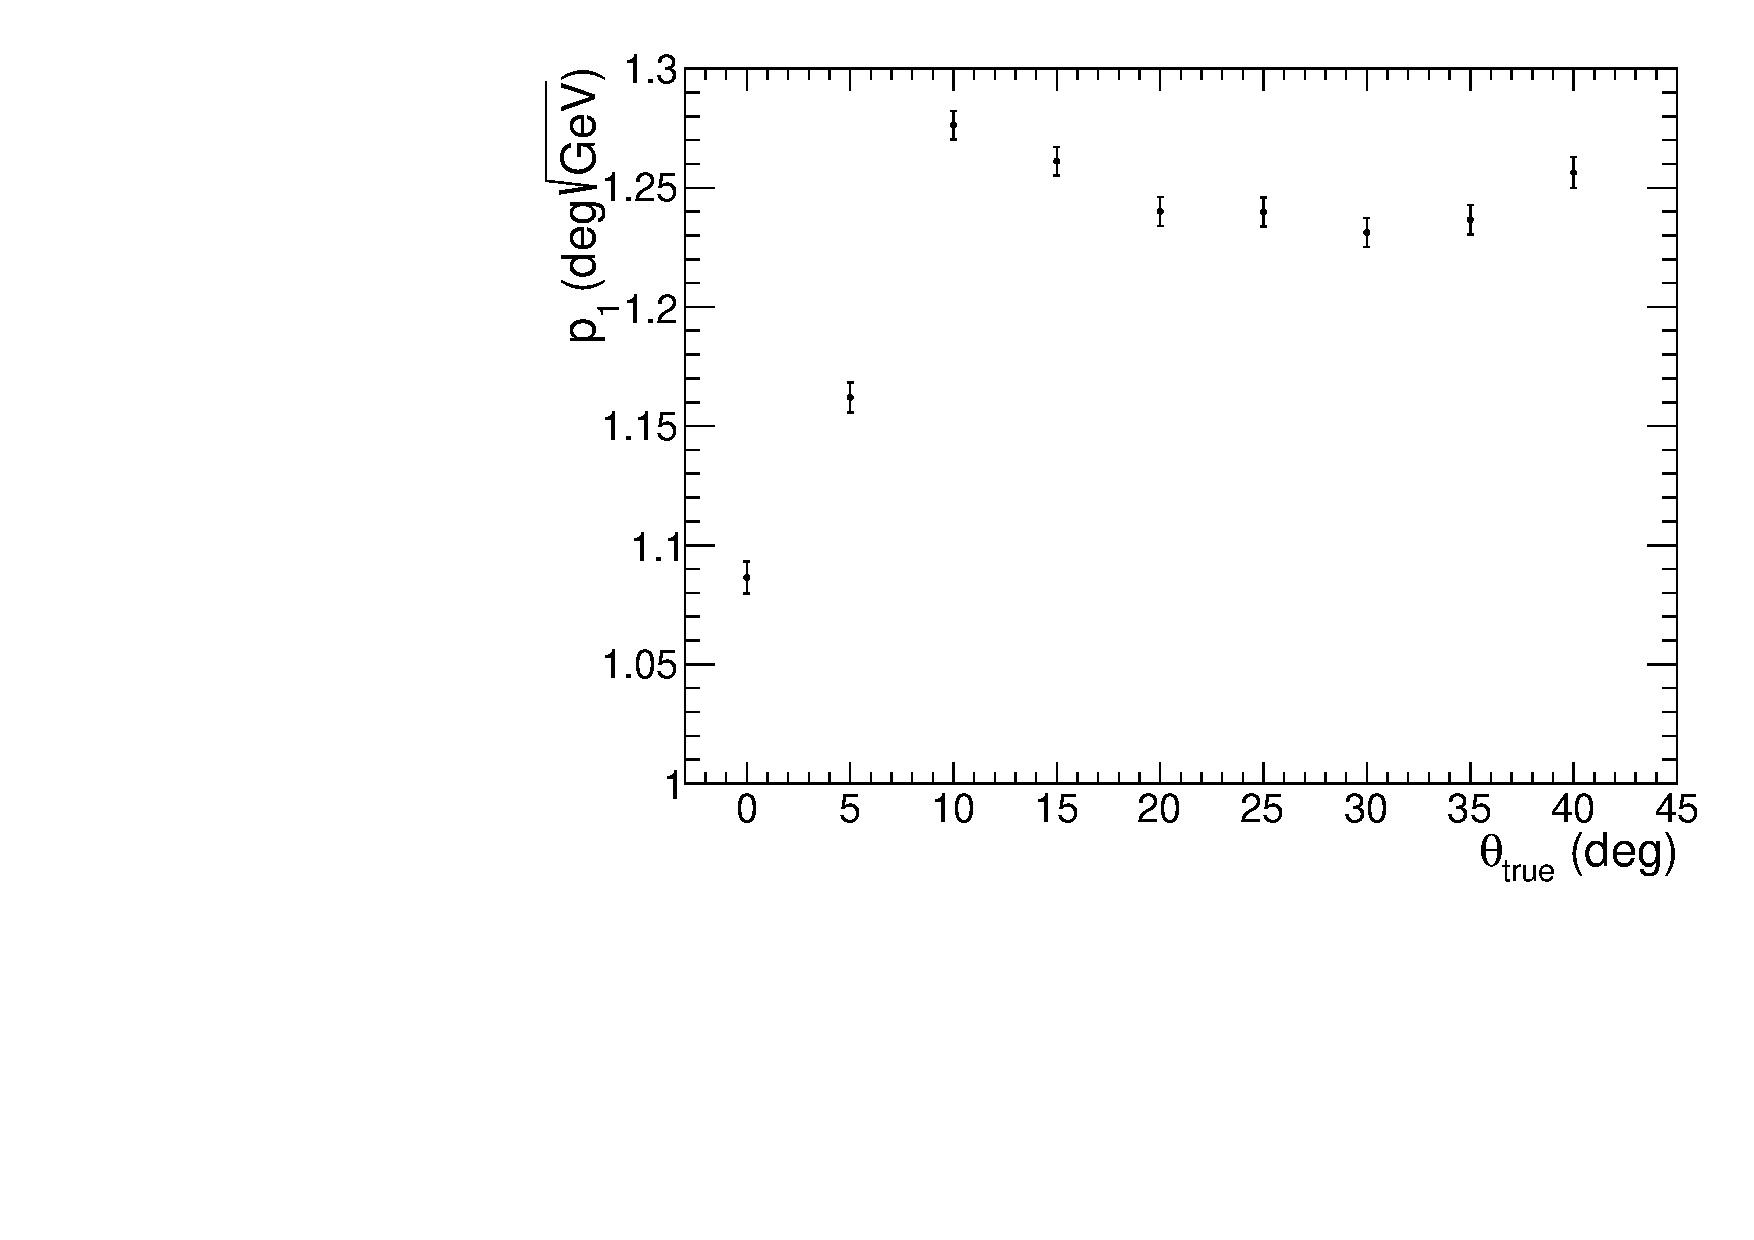
\includegraphics[width=0.44\textwidth]{figures/Fig7_p1.pdf}
\caption{ $p_{0}$ and $p_{1}$ as functions of the incident angle }
\label{fig:res_edep}
\end{figure}

Figure~\ref{fig:res_edep} shows the estimated $p_{0}$ and $p_{1}$ as functions of the incident angle. The average values of $p_{0}$ and $p_{1}$ are estimated to be 0.24$^{\circ}$ and 1.24$^{\circ}$, respectively, for $\theta>$~10$^{\circ}$. For a small $\theta$, $p_{1}$ is smaller than that for a larger $\theta$ because the angular resolution is largely dependent on the incident angle for low incident energies, whereas the opposite trend can be observed for $p_{0}$.

\begin{figure}[!hbt]
\centering
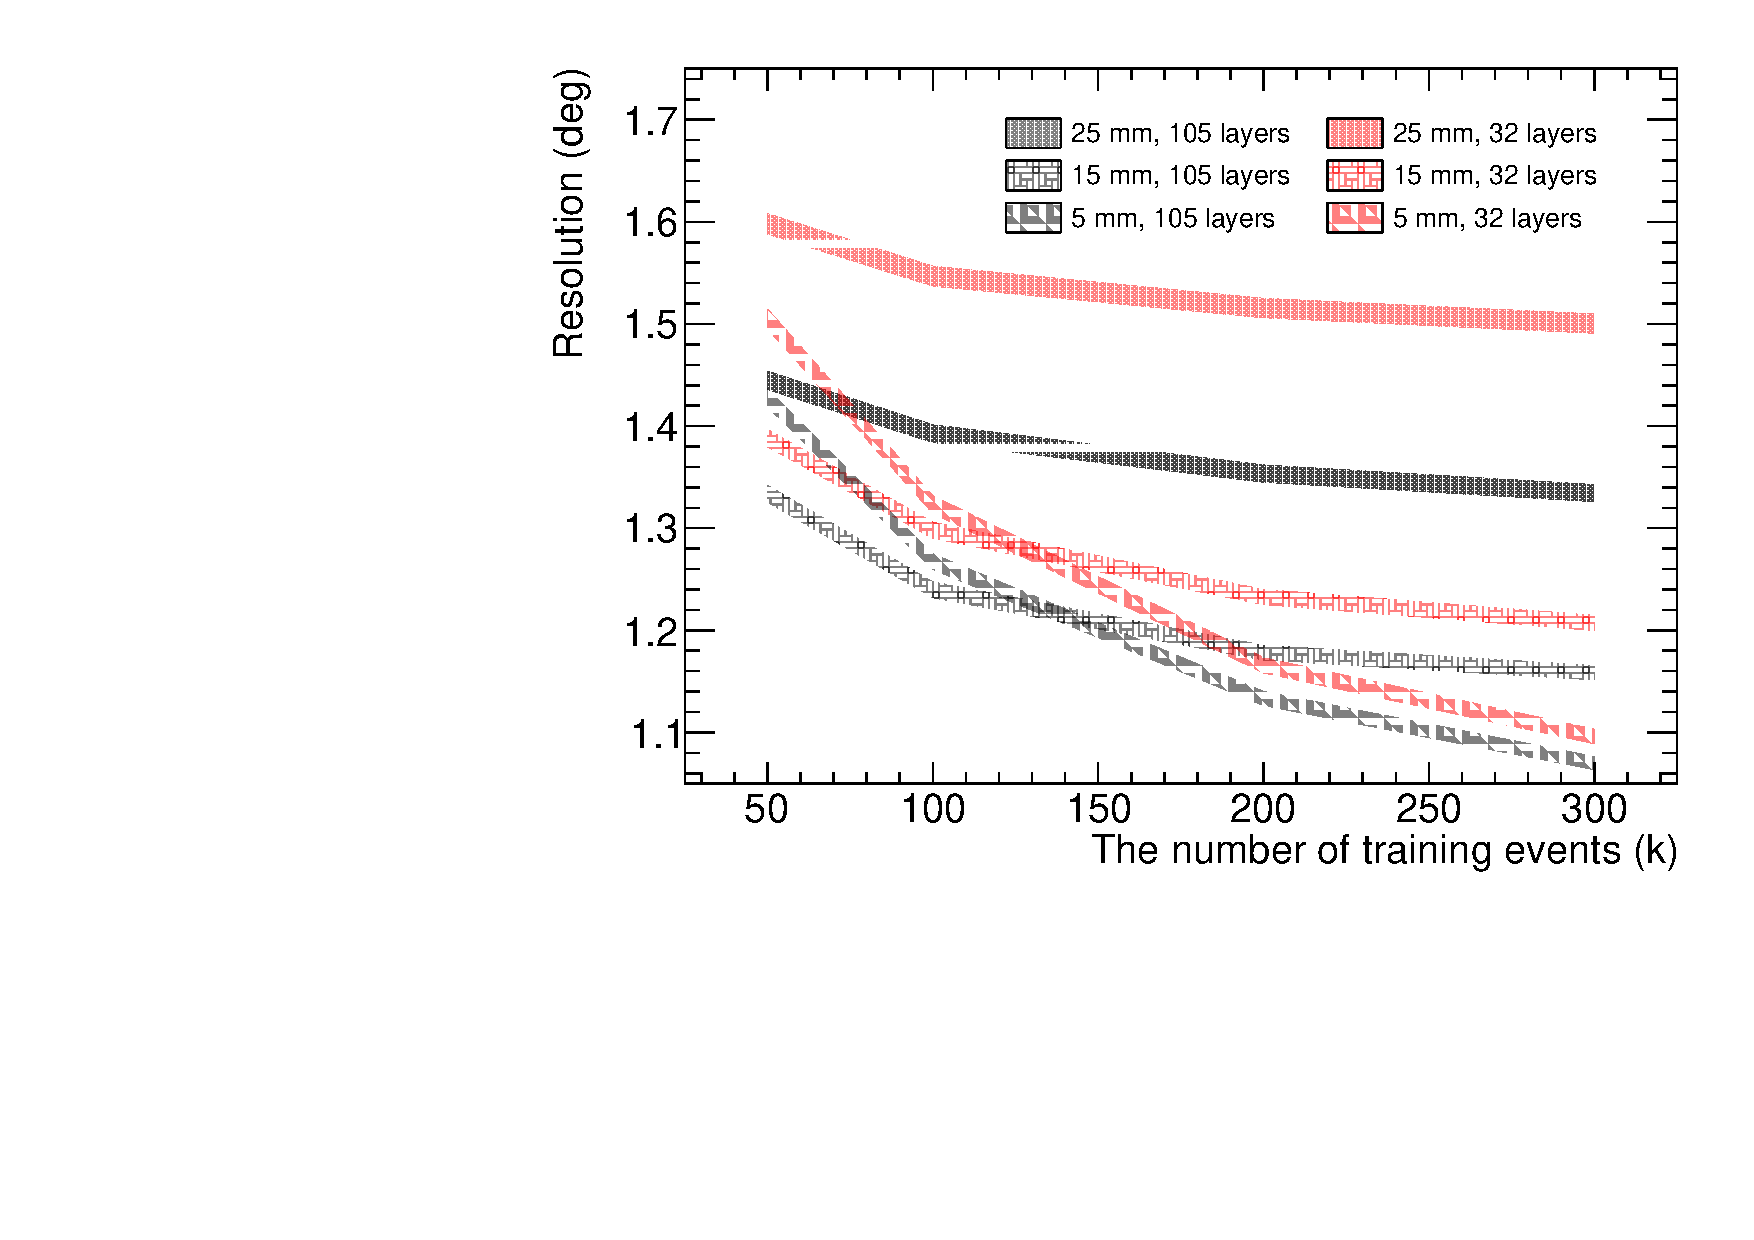
\includegraphics[width=0.6\textwidth]{figures/Fig8_nsample.pdf}
\caption{ The angular resolution for 1-GeV photons at $\theta=$~10$^{\circ}$ as a function of the number of training samples with different strip widths obtained using the first 32 layers or the full layers. }
\label{fig:multi-parameter}
\end{figure}

Figure~\ref{fig:multi-parameter} shows the angular resolution for different numbers of training samples and different detector configurations. All configurations show improvement in the angular resolution with increasing training samples, which indicates that the maturity of machine learning is an important factor in angle reconstruction. With an increase in the number of training events, the Angular resolution improves most rapidly for the configuration with 5-mm-wide scintillator strips. In other words, the required training events must be sufficiently large to correlate a larger number of features. Considering the limited computing resources, the configuration of 32 layers and 15-mm-wide strip with $10^{5}$ training events was chosen to train the XGB model. The training result for such a configuration differs by only 0.2$^{\circ}$ from that of the setup with full layers, 5-mm-wide strips, and $5\times10^{5}$ training events.
 
\section{Summary}
\label{sec:sum}

We report the simulation results of the incident angle reconstruction of EM sampling calorimeters with photons in the range of 0.1 to 2~GeV. ~To improve the angular resolution, we tuned the hyperparameters of XGBoost while considering the correlating effects among them.

In terms of detector configuration, strips with narrower widths provide better angular resolution using a finely measured EM shower with the assumption that the training is fully conducted. However, the configuration with a smaller strip width causes a larger feature size, which negatively affects the training depending on the quantity of training data. The angular resolution may be optimized by considering the two competing effects of the strip width and quantity of training data. We dedicated the front layers of the detector to reconstructing the incident angle. We obtain an angular resolution of 1.30~$\pm$~0.01$^{\circ}$ for the configuration of 32 layers (6.2$X_{0}$) of 15-mm-wide strips, which is a reduction of 0.1$^{\circ}$ compared to that of the configuration with full layers (20$X_{0}$) in the case of $10^{5}$ training samples. 

The angular resolution depends on the incident energy of the photon, and the dependence is expressed as $p_{0} \oplus p_{1}/\sqrt{E_{\gamma}}$. Except for small incident angles ($\theta<$~15~deg), the two parameters do not significantly change up to 
$40^{\circ}$, and the dependence is estimated to be 0.24 $\oplus$ 1.24$^{\circ}/\sqrt{E_{\gamma}}$. 

\label{sec:con}

%\pagebreak


\section*{Acknowledgment}
This work was supported by the National Research Foundation of Korea (NRF) 
(Grants No. 2019R1A2C1084552, 2022R1A5A1030700, and 2020R1A3B2079993) and JSPS KAKENHI Grant No. JP21H01118.
%%%the Ministry of Education, Culture, Sports, Science, and Technology (MEXT) of Japan and the Japan Society for the Promotion of Science (JSPS) under the MEXT KAKENHI Grant No. JP21H01118.

\begin{thebibliography}{99}
 
\bibitem{KOTO:MB}
Y. Tajima {\it et al.}, Nucl. Instrum. Meth. A 592, 261 (2008).

\bibitem{CMS:EMCAL}
Giovanni Mazza {\it et al.} (CMS Collaboration), Nucl. Instrum. Meth. A 958 (2020)

\bibitem{BELLE:EMCAL}
K. Miyabayashi {\it et al.}, JINST 9 (2014) 09, P09011

\bibitem{Murayama:2020mcp}
R. Murayama {\it et al.}, Nucl. Instrum. Meth. A 953 (2020) 
 
\bibitem{trk:ref}
O. Adriani {\it et al.}, Nucl. Instrum. Meth. A 854 (2017) 

\bibitem{xgboost:2016}
C. Tianqi {\it et al.}, 
{\it Proceedings of the 22nd ACM SIGKDD International Conference on Knowledge Discovery and Data Mining},
(2016) 785.

\bibitem{GGfun}
D. Gonzalez {\it et al.}, IEEE Trans. Image Processing. 4, 485 (2007)

\bibitem{GEANT4}
S. Agostinelli {\it et al.},  Nucl. Instr. and Meth. A {\bf 506} (2003) 250.

\end{thebibliography}

%\section*{Acknowledgement}
%This paper was supported by the National Research Foundation of Korea (NRF) grants funded by the Korea government (MIST) (2019R1A2C1084552 and \\ 2020R1A3B2079993).

%\bibliographystyle{elsarticle-num}
%\bibliography{paper.bib}

%\printbibliography

\end{document}

